% -------------------------------
% Plantilla del documento de proyecto en la Cátedra Ingeniería en Sistemas de Información. Versión 1.0 
%
% Sede Regional Brunca
% 
% Compilar con XeLaTeX 
% -------------------------------
\documentclass[12pt, a4paper, oneside]{book}

% -------------------------------
% Información y opciones del documento. Debe editarse.
% -------------------------------

% -------------------------------
% Configuración del documento, paquetes, etc. 
% -------------------------------
% -------------------------------
% Plantilla del Anteproyecto en la Sede Regional Brunca. Versión 0.0 (Preliminar)
%
% CTFG Sede Regional Brunca
% 
% Compilar con XeLaTeX 
% -------------------------------


% -------------------------------
% Idioma
% -------------------------------
\usepackage{polyglossia}
\setmainlanguage{spanish}


% -------------------------------
% Fuente
% -------------------------------
% Cualquier tamaño de texto: {\fontsize{100pt}{120pt}\selectfont tutexto}
\usepackage{anyfontsize}
% Selección de fuentes.
\usepackage{fontspec}
% Espacio entre líneas
\usepackage{setspace}
% Fuentes especiales
\usepackage{textcomp,marvosym,pifont}


% -------------------------------
% Otros paquetes de uso común
% -------------------------------
% Símbolos matemáticos
\usepackage{amsmath,amsfonts,amssymb}
% Gráficos
\usepackage{graphicx}
% Posición arbitraria de los gráficos
\usepackage[absolute,overlay]{textpos}
% Apéndices
\usepackage{appendix}


% -------------------------------
% Esquema de colores
% -------------------------------
% Paquete para la definición de colores
\usepackage[table]{xcolor}
% Esquema de colores
\input{include/colores}


% -------------------------------
% Márgenes
% -------------------------------
% Márgenes de las páginas
\usepackage[
	inner	 =	3cm,   % Margen interior
	outer	 =	2.5cm, % Margen exterior
	top	 =	2.5cm, % Margen superior
	bottom =	2.5cm, % Margen inferior
	includeheadfoot, % Incluye cabecera y pie de página en los márgenes
]{geometry}
% Muestra una regla para comprobar el formato de las páginas (descomentar)
%\usepackage[type=upperleft,showframe,marklength=8mm]{fgruler} 


% -------------------------------
% Renombra tablas y bibliografía
% -------------------------------
\addto\captionsspanish{
	\renewcommand{\listtablename}{Índice de tablas}
	\renewcommand{\tablename}{Tabla}
	\renewcommand{\bibname}{Referencias bibliográficas}
}


% -------------------------------
% Itemize y enumerate. Control de los espacios.
% -------------------------------
\usepackage{enumitem}
\setitemize{itemsep=0pt}
\setenumerate{itemsep=0pt}
\renewcommand{\labelitemi}{\tiny\bft{$\blacksquare$}}
\renewcommand{\labelitemii}{\bft{$\bullet$}}
\renewcommand{\labelitemiii}{\bft{-}}


% -------------------------------
% Enlaces y colores
% -------------------------------
\usepackage{hyperref}
%\hypersetup{
%    colorlinks,
%    citecolor=black,
%    filecolor=black,
%    linkcolor=black,
%    urlcolor=black
%}

% -------------------------------
% Gestión de elementos flotantes
% -------------------------------
% Para forzar a que las figuras aparezcan antes del fin de una sección.
%\usepackage[section]{placeins}

% Gestión de títulos de los elementos flotantes
\usepackage{caption}
% Subfiguras y títulos en subfiguras
\usepackage{subcaption}

% Títulos
\DeclareCaptionFont{tema}{\color{tema}} % Color
\captionsetup{labelfont={tema, bf}}     % Estilo
\captionsetup{font=normalsize}          % Tamaño
\captionsetup{width=.9\linewidth}       % Anchura del título
% Distancia de la figura al texto.
\setlength{\intextsep}{1cm}
\setlength{\textfloatsep}{1cm}


% -------------------------------
% Utilidades para tablas
% -------------------------------
% Para fundir filas en tablas
\usepackage{multirow}
% Para definir columnas con ancho fijo y alineación
\usepackage{array,ragged2e}
\newcolumntype{L}[1]{>{\raggedright\let\newline\\\arraybackslash\hspace{0pt}}m{#1}}
\newcolumntype{C}[1]{>{\centering\let\newline\\\arraybackslash\hspace{0pt}}m{#1}}
\newcolumntype{R}[1]{>{\raggedleft\let\newline\\\arraybackslash\hspace{0pt}}m{#1}}


% -------------------------------
% Para tabular
% -------------------------------
\usepackage{tabto}


% -------------------------------
% Formato de títulos, capítulos, etc.
% -------------------------------
\usepackage{titlesec, titletoc}
% Parte
\titleformat{\part}[display]												   	   % Estilo
{\Huge \centering \color{tema}}                                                % Formato
{Parte \thepart }                                                              % Etiqueta
{0.75ex}                                                                       % Separación
{\bfseries\fontsize{25pt}{40pt}\selectfont}                                    % Entre etiqueta y título            
[\thispagestyle{empty}]                                                        % Después

% Capítulo		
\titleformat{\chapter}[block]            			 			                    % Estilo  	
{\vspace{0cm} \flushright \bfseries \LARGE \color{tema}}  	        			% Formato 
{\thechapter.}                  			  									% Etiqueta
{0.75ex}                                     									% Separación
{}                                           									% Entre etiqueta y título
[\vspace{0.1cm} \rule{0.5\textwidth}{1pt}\vspace*{1cm}\thispagestyle{plain}]    % Después      

% Sección
\titleformat{\section}
{\vspace{5pt}  \Large \color{tema}}
{\thesection .}
{0.75ex}
{}

% Subsección
\titleformat{\subsection}
{\large \color{tema}}
{\thesubsection .}
{0.75ex}
{}

% Subsubsección
\titleformat{\subsubsection}
{\bf\color{tema}}
{}
{0.75ex}
{}

% Parte (TOC)
\titlecontents{part}[2pc]
{\vspace{20pt}\bfseries\filright\Large\color{tema}}
{\contentslabel{1.5pc}}{\hspace*{-1.5pc}}
{\vspace{5pt}}
{}

% Capítulo (TOC)
\titlecontents{chapter}[2pc]
{\vspace{10pt}\bfseries\large\filright}
{\contentslabel{1.5pc}}{\hspace*{-1.5pc}}
{\mdseries\titlerule*[0.5pc]{.}\bfseries\contentspage}

% Sección (TOC)
\titlecontents{section}[4pc]
{\vspace{5pt}\filright}
{\contentslabel{2pc}}{\hspace*{2pc}}
{\titlerule*[0.5pc]{.}\contentspage}
{\vspace{5pt}

	% Subsección (TOC)
	\titlecontents{subsection}[6pc]
	{\vspace{2.5pt}\filright\small\em}
	{\contentslabel{3pc}}{\hspace*{-3pc}}
	{\titlerule*[0.5pc]{.}\contentspage}}


% -------------------------------
% Cabeceras y pie de página
% -------------------------------
\usepackage{fancyhdr}

\pagestyle{fancy}
\fancyhf{} % Limpiar todas las cabeceras y pies de página

% Definir el nombre de la empresa
\newcommand{\nombreempresa}{Café y Vivero Verde Pradera}

% Pie de página centrado con el nombre de la empresa
\fancyfoot[C]{\nombreempresa}

% Cabecera con el nombre del capítulo a la izquierda
\fancyhead[L]{\leftmark}  % Título del capítulo
\fancyhead[R]{\thepage}   % Número de página

% Ajuste de las líneas de cabecera y pie de página
\renewcommand{\headrulewidth}{0.5pt}  % Línea en la cabecera
\renewcommand{\footrulewidth}{0.5pt}  % Línea en el pie de página

% Redefinición del estilo de página 'plain' para capítulos y partes
\fancypagestyle{plain}{
	\fancyhf{}  % Limpiar cabeceras y pies de página
	\fancyfoot[LE,RO]{\thepage} % Número de página a la izquierda en páginas pares, derecha en impares
	\fancyfoot[C]{\nombreempresa}  % Nombre de la empresa en el pie de página
	\renewcommand{\headrulewidth}{0pt}  % Sin línea en la cabecera
	\renewcommand{\footrulewidth}{0.5pt}  % Línea en el pie de página
}

% -------------------------------
% Utilidades
% -------------------------------
% Marcas
\newcommand{\pcite}{\bfr{[?]}\,} % Cita pendiente: [?] en rojo y negrita.
\newcommand{\ps}{\bfr{[-}\,} % Pricipio de un bloque en sucio
\newcommand{\fs}{\bfr{-]}\,} % Fin de un bloque en sucio.

% Notas
\usepackage[textsize=tiny,spanish,shadow,textwidth=2cm]{todonotes}

% Para generar textos "random"
\usepackage{lipsum}




% -------------------------------
% Algoritmos y código
% -------------------------------

% Se definen entornos específicos para algoritmos y código que permiten
% gestionar los títulos manera similar en ambos casos, y similar al resto
% de elementos flotantes.
\usepackage{newfloat}

% Define un estilo para el encabezado de algoritmos y código.
\DeclareCaptionFormat{algcode}{
	\rule{\dimexpr\textwidth\relax}{1pt}\vspace{0.2cm}
	#1#2#3
	\rule{\dimexpr\textwidth\relax}{1pt}
}
\captionsetup[algorithm]{format=algcode, width=\linewidth}
\captionsetup[code]{format=algcode, width=\linewidth}


% -------------------------------
% Caracteres pifont de uso común (con color)
% -------------------------------
\newcommand{\vmarkt}{\textcolor{tema}{\ding{52}} }  % Checked (V) Tema
\newcommand{\vmarkr}{\textcolor{rojo}{\ding{52}} }  % Checked (V) Rojo
\newcommand{\vmarka}{\textcolor{azul}{\ding{52}} }  % Checked (V) Azul

\newcommand{\xmarkt}{\textcolor{tema}{\ding{55}} }  % Checked (X) Tema
\newcommand{\xmarkr}{\textcolor{rojo}{\ding{55}} }  % Checked (X) Rojo
\newcommand{\xmarka}{\textcolor{azul}{\ding{55}} }  % Checked (X) Azul

\newcommand{\lmarkt}{\textcolor{tema}{\ding{46}} }  % Lápiz Tema
\newcommand{\lmarkr}{\textcolor{rojo}{\ding{46}} }  % Lápiz Rojo
\newcommand{\lmarka}{\textcolor{azul}{\ding{46}} }  % Lápiz Azul

\newcommand{\hmarkt}{\textcolor{tema}{\ding{43}} }  % Mano Tema
\newcommand{\hmarkr}{\textcolor{rojo}{\ding{43}} }  % Mano Roja 
\newcommand{\hmarka}{\textcolor{azul}{\ding{43}} }  % Mano Azula 

\newcommand{\fmarkt}{\textcolor{tema}{\ding{220}} }  % Flechza Tema
\newcommand{\fmarkr}{\textcolor{rojo}{\ding{220}} }  % Flecha Roja 
\newcommand{\fmarka}{\textcolor{azul}{\ding{220}} }  % Flecha Azul
\usetikzlibrary{positioning, arrows.meta, shadows, calc}

% Documento
\begin{document}

% -------------------------------
% Portada y título
% -------------------------------
% Fuente  de la portada
% \setmainfont[Ligatures={NoRequired,NoCommon,NoContextual}]{Calibri}
% -------------------------------
% Plantilla del Anteproyecto en la Sede Regional Brunca. Versión 0.0 (Preliminar)
%
% CTFG Sede Regional Brunca
% 
% Compilar con XeLaTeX 
% -------------------------------
\pagestyle{empty}
\begin{titlepage}\null



\begin{textblock*}{\paperwidth}(0cm,4cm)
\begin{center}
\begin{figure}[ht]    \centerline{
\includegraphics[scale=0.4]{figs/logo_una.jpg}}
\end{figure}
\end{center}
\end{textblock*}


\begin{textblock*}{\paperwidth}(0cm,9cm) 
\begin{center}\doublespacing
{\fontsize{16pt}{2pt}\selectfont Universidad Nacional de Costa Rica}

{\fontsize{16pt}{2pt}\selectfont Sede Regional Brunca}

{\fontsize{16pt}{2pt}\selectfont Campus PZ - Coto}
\end{center}


\end{textblock*}


\begin{textblock*}{\paperwidth}(0cm,13.5cm) 
\begin{center}\doublespacing 
{\bf\fontsize{18pt}{4pt}\selectfont Cátedra Ingeniería Sistemas}

{\fontsize{16pt}{4pt}\selectfont Bachillerato en Ingeniería en Sistemas de Información}
\end{center}
\end{textblock*}


% El título ocupa el 80% de la página. Puede adaptarse 
% a la longitud del texto
\begin{textblock*}{0.8\paperwidth}(0.1\paperwidth,18cm) 
\begin{center}\doublespacing % onehalfspace

\vskip1cm
\end{center}
\end{textblock*}


\begin{textblock*}{\paperwidth}(0cm,25.5cm) 
\begin{center}
\end{center}
\end{textblock*}
\end{titlepage}

% -------------------------------
% Fuente del documento.
% -------------------------------
% La fuente recomendada es Calibri, pero no está instalada en overleaf:
%\setmainfont[Ligatures={NoRequired,NoCommon,NoContextual}]{Calibri}

% Para utilizarla aquí, son necesarios los archivos .ttf correspondientes:
%\setmainfont[
%			BoldFont=Calibrib.ttf,
%			ItalicFont=Calibrii.ttf,
%			BoldItalicFont=Calibriz.ttf
%		]{Calibri.ttf}

% Por defecto, utiliza una fuente instalada en overleaf. 
% Éstas son algunas que van bien con la plantilla:
%\setmainfont{Alegreya Sans} 
%\setmainfont{Carlito}
%\setmainfont{PT Sans}
%\setmainfont{Source Sans Pro}

% -------------------------------
% Índices y tablas
% -------------------------------
\tableofcontents	% Índice
\listoffigures		% Índice de figuras
\listoftables		% Índice de tablas
%\cleardoublepage
%\newpage
% -------------------------------
% Documento
% -------------------------------
\mainmatter
% Estilo de página
\pagestyle{fancy}

% Capitulos del documento

\chapter{Introducción} 

El presente documento detalla exhaustivamente el proceso de investigación y desarrollo 
llevado a cabo en el proyecto de fin de carrera de los estudiantes del programa de 
Ingeniería en Sistemas de Información de la Universidad Nacional de Costa Rica. 
Este proyecto se centra en la creación e implementación de soluciones de software 
innovadoras, diseñadas para equipar a los estudiantes con las habilidades necesarias 
para enfrentar los desafíos del entorno laboral actual en tecnologías de la información.

El objetivo primordial es proporcionar una experiencia práctica y relevante de integración en 
escenarios reales de trabajo, promoviendo así el desarrollo de competencias críticas como 
el análisis de problemas, diseño de sistemas, programación avanzada, gestión de proyectos y 
colaboración interdisciplinaria. A través de este enfoque, el proyecto no solo pretende 
reforzar el conocimiento teórico adquirido durante el curso académico, sino también fomentar 
la innovación y la creatividad en la solución de problemas complejos.

Asimismo, este documento expone los criterios metodológicos adoptados, incluyendo las fases 
de planificación, ejecución y evaluación del proyecto. Se describen las herramientas y tecnologías 
seleccionadas, justificando su uso en base a las tendencias actuales del mercado y su relevancia 
para los objetivos de aprendizaje del programa. Además, se discuten los resultados obtenidos, 
proporcionando análisis y conclusiones que destacan la contribución del proyecto al desarrollo 
profesional de los estudiantes.

En resumen, este documento sirve como un archivo comprensivo del trabajo realizado, también como un
 recurso formativo que guía a los estudiantes en la aplicación efectiva 
de sus habilidades técnicas en el mundo real, preparándolos para contribuir significativamente en 
sus futuros roles como profesionales de sistemas de información.

\chapter{Capítulo II: Metodología}
\section{Metodología}
Para el desarrollo del sistema de gestión de nóminas para Café y
Vivero Verde Pradera, se empleará una combinación de metodologías ágiles,
específicamente el Desarrollo Incremental y Scrum. Esta combinación está
diseñada para adaptarse a la naturaleza dinámica del proyecto y facilitar
la colaboración continua con los usuarios finales.

\subsection{Fundamentación}

El Desarrollo Incremental permite la construcción del sistema en
múltiples ciclos o incrementos. Cada incremento agrega funcionalidad y
es plenamente operativo, lo que posibilita la entrega de una versión mejorada
del sistema con cada iteración. Esta metodología es particularmente efectiva
para obtener retroalimentación temprana y continua de los usuarios, permitiendo
ajustes que alinean el producto final con las necesidades específicas del cliente.

Por otro lado, Scrum se empleará para gestionar y planificar el proceso de
desarrollo. Scrum es un marco de trabajo que promueve la comunicación frecuente,
el trabajo en equipo, y la flexibilidad para adaptarse a cambios. Las ceremonias
de Scrum, como las reuniones diarias (Daily Scrum), las revisiones de sprint y
las planificaciones (Sprint Planning), facilitarán la coordinación y el
seguimiento constante del avance del proyecto.

\newpage

\subsection{Aplicación en el Proyecto}


En la aplicación práctica de estas metodologías en el proyecto:
\begin{itemize}
	\item \textbf{Planificación Scrum:} Se establecerán sprints de duración fija,
	      ya sea mensual o quincenal, durante los cuales se definirán objetivos
	      claros y alcanzables. Esto incluirá la definición de las funcionalidades
	      a desarrollar, pruebas y revisiones con los usuarios finales.
	\item \textbf{Desarrollo Incremental:} Cada sprint resultará en un
	      incremento funcional del sistema, que será evaluado por los usuarios finales.
	      La retroalimentación recogida será utilizada para mejorar o ajustar las
	      funcionalidades en los siguientes incrementos.
	\item \textbf{Cambios mínimos:} Se ajustará la duración de los sprints según
	      la complejidad de las funcionalidades y la capacidad del equipo de desarrollo,
	      buscando el equilibrio óptimo para una entrega eficiente y efectiva.
\end{itemize}





Con estas metodologías, el proyecto no solo apuntará a cumplir con los objetivos establecidos de manera eficaz, sino que también se adaptará a las necesidades cambiantes del entorno y los usuarios finales, asegurando la entrega de un sistema que verdaderamente responda a las expectativas y requerimientos de la empresa Café y Vivero Verde Pradera.

\subsection{Definición de estandares a utilizar}

En este apartado, describiremos los estándares seleccionados para cada una 
de las áreas clave del desarrollo del software, asegurando la consistencia, 
claridad y eficacia en la implementación y mantenimiento del proyecto.

\subsection{\textbf{Estándares de Documentación}}

Adoptaremos prácticas de documentación de código fuente, incluyendo comentarios detallados, 
encabezados de archivos y documentación exhaustiva de la API, para facilitar el entendimiento 
y la mantenibilidad del código. La documentación seguirá guías de estilo rigurosas que promueven
la claridad y un formato coherente en todos los documentos técnicos y manuales de usuario, 
asegurando que toda la información sea accesible y comprensible para todos los interesados.

Los comentarios deben realizarse de la siguiente manera:
\begin{itemize}
    \item \textbf{Bloque de comentarios:} Para explicar la funcionalidad de los métodos.
    \item \textbf{Línea de comentario:} Solo para la declaración de variables o en líneas de 
    código donde sea necesaria una especificación.
\end{itemize}

\subsection{\textbf{Estándares de Programación}}

Estableceremos convenciones de nombramiento para variables, clases y métodos en 
inglés que reflejen claramente su función. Utilizaremos un formato de indentación que 
facilite la lectura del código y mantendremos las líneas de código a una longitud razonable 
para evitar la complejidad visual. Emplearemos Git como sistema de control de versiones, con un 
esquema de nomenclatura de commits que incluye etiquetas como \texttt{[ADDED]}, \texttt{[BUG]}, 
\texttt{[FIXED]}, \texttt{[UPDATED]}, y \texttt{[FEATURE]}, acompañados de comentarios precisos 
que describan los cambios realizados. Además, incluiremos el uso de pull requests en GitHub para 
evitar conflictos en el desarrollo del software. Se prohibirá el uso de push forzados y la 
agregación de todos los archivos simultáneamente, a menos de que hayan sido modificados 
por la misma razón. Implementaremos revisiones de código entre pares y utilizaremos 
herramientas como VS Code Insiders con GitHub Copilot para realizar pruebas automáticas.

La estructura del proyecto se organizará de la siguiente manera: 
\begin{itemize}
    \item \textbf{Design:} Donde se incluirá el diseño de cada una de las pantallas a usar.
    \item \textbf{Docs:} Donde se almacenarán todos los documentos del sistema, como guías 
    de usuario y documentos de investigación.
    \item \textbf{Source:} Que contendrá el código fuente del sistema, distribuido en:
    \begin{itemize}
        \item \textbf{DB:} Que incluirá el diagrama de base de datos, el esquema de la 
        base de datos y el SQL de la base de datos.
        \item \textbf{API:} Donde se almacenará todo el código relacionado con la API.
        \item \textbf{ENV:} Que contendrá las variables de entorno.
        \item \textbf{Front-End:} Donde se incluirá todo lo relacionado con la parte frontal 
        del sistema.
        \item \textbf{Back-End:} Que contendrá todo lo relacionado con el backend del sistema.
    \end{itemize}
\end{itemize}

\subsection{\textbf{Estándares de Bases de Datos}}

Las definiciones de tablas y columnas seguirán un esquema de nomenclatura específico, 
donde las tablas comenzarán con \texttt{VPG\_} seguido del nombre de la tabla en mayúsculas, 
y las columnas se nombrarán en minúsculas siguiendo el formato \texttt{tablename\_atributo}. 
Las relaciones se nombrarán siguiendo el formato \texttt{VPG\_TABLENAME1\_TABLENAME2\_FK}. 
Adheriremos a las tres primeras reglas de normalización para garantizar una estructura de 
base de datos eficiente y optimizada tanto para consultas como para la integridad de los datos.

\subsection{\textbf{Estándares de Interfaz}}

Las interfaces seguirán una guía de estilo que incluye el uso de colores no muy 
llamativos basados en los colores de la empresa y la tipografía INTER para garantizar 
una presentación visual coherente y profesional. La disposición de los elementos estará a 
cargo del diseñador web, con un fuerte enfoque en la accesibilidad para cumplir con las 
directrices de WCAG. Además, fomentaremos la reutilización de componentes para maximizar la 
eficiencia del desarrollo. Las pruebas de interfaz se realizarán mediante evaluaciones 
entre compañeros y con feedback directo de los usuarios finales de la empresa, asegurando 
que las interfaces sean intuitivas y efectivas.

Estos estándares son fundamentales para el desarrollo exitoso del software, proporcionando un 
marco de trabajo claro y eficiente para todo el equipo del proyecto. Sin embargo, siempre habrá 
un espacio para revisar y adaptar las políticas conforme el proyecto crezca y cambie.
\chapter{\textbf{Capitulo III: Análisis}}

\section{Análisis Preliminar}

Para el cálculo de la nómina, actualmente se cuenta con un dispositivo lector de huella digital en el cual los colaboradores registran su ingreso y salida de su jornada laboral. Esta información es extraída manualmente por el personal administrativo y luego procesada en hojas de cálculo, lo cual representa una tarea operativa repetitiva, propensa a errores humanos y sin integración con otros procesos internos.

Aunque existe un mecanismo básico de registro de jornada, la ausencia de un sistema que centralice y automatice el procesamiento de dicha información genera cuellos de botella en actividades como la emisión de reportes, la gestión de eventos laborales (vacaciones, incapacidades, permisos especiales), y la elaboración de comprobantes de pago.

Este análisis evidencia la necesidad de optimizar el flujo de información ya disponible en el entorno organizacional, de modo que pueda ser aprovechada de forma estructurada y confiable mediante una solución tecnológica que integre las funcionalidades necesarias para mejorar la eficiencia y la trazabilidad del proceso.

\subsection{Gestión de Riesgos}

La gestión de riesgos es un proceso fundamental para identificar, evaluar y controlar los posibles eventos que pueden afectar el éxito del proyecto. A continuación, se presenta la identificación de riesgos, la matriz de probabilidad por impacto para priorizarlos, y el plan de tratamiento de riesgos propuesto para el desarrollo del sistema de gestión de nómina para Café y Vivero Verde Pradera.

\subsubsection*{Identificación de Riesgos}

Durante el análisis del proyecto se identificaron los siguientes riesgos relevantes que pueden afectar su desarrollo y operación:

\begin{itemize}
	\item \textbf{Fallos de integración tecnológica:} Problemas al conectar el reloj marcador con el sistema de nómina que pueden ocasionar errores en los datos de asistencia.
	\item \textbf{Fallas en la conectividad:} Interrupciones en el servicio de internet que impidan el acceso remoto y afecten la continuidad del sistema.
	\item \textbf{Errores de programación:} Bugs o fallos en el software que comprometan la funcionalidad de los módulos críticos.
	\item \textbf{Incompatibilidad tecnológica:} Desajustes entre las versiones de hardware y software utilizados.
	\item \textbf{Capacitación insuficiente:} Falta de entrenamiento adecuado para los usuarios finales que dificulte el uso correcto del sistema.
	\item \textbf{Resistencia al cambio:} Oposición del personal a adoptar nuevas tecnologías y procesos digitales.
	\item \textbf{Errores humanos:} Fallos en la entrada o manejo de datos por falta de experiencia o atención.
	\item \textbf{Limitaciones presupuestarias:} Recursos económicos insuficientes para la adquisición de hardware, licencias o capacitación.
	\item \textbf{Retrasos en pagos a proveedores:} Problemas en el flujo de caja que afecten la entrega de insumos y servicios.
	\item \textbf{Incumplimiento normativo:} Falta de adecuación a las regulaciones legales vigentes.
	\item \textbf{Riesgos en protección de datos:} Posibles vulneraciones a la privacidad y seguridad de la información sensible.
	\item \textbf{Desastres naturales:} Eventos que puedan afectar la infraestructura tecnológica o los datos almacenados.
\end{itemize}

\subsubsection*{Matriz de Probabilidad por Impacto}

Para priorizar los riesgos identificados, se evaluó la probabilidad de ocurrencia y el impacto que tendría cada uno en el proyecto, multiplicando ambos factores para obtener un nivel de riesgo cuantificado. La siguiente tabla presenta esta matriz:

\begin{table}[h!]
	\centering
	\begin{tabular}{|l|c|c|c|}
		\hline
		\textbf{Riesgo}                & \textbf{Probabilidad} & \textbf{Impacto} & \textbf{Nivel de Riesgo} \\ \hline
		Fallos de integración          & Media (3)             & Alto (5)         & 15                       \\ \hline
		Fallas de conectividad         & Baja (2)              & Medio (4)        & 8                        \\ \hline
		Errores de implementación      & Alta (4)              & Alto (5)         & 20                       \\ \hline
		Compatibilidad tecnológica     & Media (3)             & Medio (3)        & 9                        \\ \hline
		Capacitación inadecuada        & Media (3)             & Alto (5)         & 15                       \\ \hline
		Resistencia al cambio          & Alta (4)              & Medio (3)        & 12                       \\ \hline
		Errores humanos                & Alta (4)              & Medio (3)        & 12                       \\ \hline
		Presupuesto insuficiente       & Media (3)             & Alto (5)         & 15                       \\ \hline
		Retrasos en pago a proveedores & Baja (2)              & Medio (3)        & 6                        \\ \hline
		Cumplimiento normativo         & Media (3)             & Alto (5)         & 15                       \\ \hline
		Protección de datos            & Alta (4)              & Alto (5)         & 20                       \\ \hline
		Desastres naturales            & Baja (1)              & Alto (5)         & 5                        \\ \hline
	\end{tabular}
	\caption{Matriz de probabilidad por impacto}
	\label{tab:matriz_prob_impacto}
\end{table}
\newpage

\subsubsection*{Plan de Tratamiento de Riesgos}

Para cada riesgo, se diseñaron acciones para mitigar su probabilidad o impacto, asegurando que el proyecto pueda desarrollarse de forma controlada y segura. A continuación, se presenta el análisis detallado con las acciones propuestas:

\begin{table}[h!]
	\centering
	\resizebox{\textwidth}{!}{ % Ajusta el tamaño al ancho del texto
		\begin{tabular}{|c|l|l|p{3cm}|c|c|c|c|p{4cm}|l|c|}
			\hline
			\textbf{ID} & \textbf{Riesgo}                & \textbf{Categoría} & \textbf{Descripción}                                                                             & \textbf{Prob.} & \textbf{Impacto} & \textbf{Detec.} & \textbf{NPR} & \textbf{Plan de Tratamiento}                                         & \textbf{Responsable}      & \textbf{Estado} \\ \hline
			1           & Fallos de integración          & Técnico            & Problemas para conectar el reloj marcador con el sistema causando errores en datos de asistencia & 3              & 5                & 3               & 45           & Realizar pruebas de integración tempranas y usar APIs estandarizadas & Equipo de desarrollo      & Pendiente       \\ \hline
			2           & Fallas de conectividad         & Técnico            & Caídas en internet que impiden el acceso remoto al sistema                                       & 2              & 4                & 4               & 32           & Implementar conexiones redundantes y sistemas de respaldo            & Equipo de infraestructura & Pendiente       \\ \hline
			3           & Errores de implementación      & Técnico            & Bugs o fallos en el software que afectan módulos críticos                                        & 4              & 5                & 2               & 40           & Pruebas continuas, revisión de código y control de calidad           & Equipo de desarrollo      & Pendiente       \\ \hline
			4           & Compatibilidad tecnológica     & Técnico            & Incompatibilidad entre versiones de software o hardware                                          & 3              & 3                & 3               & 27           & Pruebas previas de compatibilidad y evaluación de versiones          & Equipo de desarrollo      & Pendiente       \\ \hline
			5           & Capacitación inadecuada        & Operativo          & Falta de entrenamiento adecuado para usuarios finales                                            & 3              & 5                & 4               & 60           & Programar formación y materiales de apoyo                            & Recursos Humanos          & Pendiente       \\ \hline
			6           & Resistencia al cambio          & Operativo          & Personal se resiste a adoptar el nuevo sistema                                                   & 4              & 3                & 4               & 48           & Involucrar a usuarios en el proceso y comunicación constante         & Gestión del proyecto      & Pendiente       \\ \hline
			7           & Errores humanos                & Operativo          & Errores en la entrada o manejo de datos por falta de experiencia                                 & 4              & 3                & 3               & 36           & Automatizar procesos y diseñar interfaces intuitivas                 & Equipo de desarrollo      & Pendiente       \\ \hline
			8           & Presupuesto insuficiente       & Financiero         & Limitaciones económicas que impiden compra de hardware o licencias                               & 3              & 5                & 4               & 60           & Planificar presupuesto con margen y negociar con proveedores         & Gestión financiera        & Pendiente       \\ \hline
			9           & Retrasos en pago a proveedores & Financiero         & Problemas en flujo de caja que retrasan entregas                                                 & 2              & 3                & 4               & 24           & Mantener comunicación constante con proveedores                      & Gestión financiera        & Pendiente       \\ \hline
			10          & Cumplimiento normativo         & Legal              & No cumplir leyes laborales o de protección de datos                                              & 3              & 5                & 3               & 45           & Revisar normativas y actualizar el sistema conforme a regulaciones   & Equipo legal/QA           & Pendiente       \\ \hline
			11          & Protección de datos            & Legal              & Riesgo de fuga o acceso no autorizado a datos personales                                         & 4              & 5                & 2               & 40           & Implementar encriptación, autenticación fuerte y auditorías          & Equipo de seguridad       & Pendiente       \\ \hline
			12          & Desastres naturales            & Ambiental          & Eventos naturales que afectan infraestructura y datos                                            & 1              & 5                & 5               & 25           & Plan de recuperación y backups en la nube                            & Equipo infraestructura    & Pendiente       \\ \hline
		\end{tabular}
	}
	\caption{Matriz de gestión de riesgos del proyecto}
	\label{tab:gestion_riesgos}
\end{table}

\newpage
\subsection{Estudio de factibilidad}

\subsubsection{Factibilidad Operativa}

\begin{itemize}
	\item \textbf{Conocimiento de los desarrolladores:} Los desarrolladores del sistema son estudiantes avanzados de Ingeniería en Sistemas, con experiencia en desarrollo web, bases de datos y metodologías ágiles, lo que garantiza una correcta implementación del proyecto.

	\item \textbf{Habilidad de los usuarios:} El sistema está orientado al personal administrativo de la empresa, quienes ya realizan los procesos manuales y tienen el conocimiento necesario para adaptarse al uso de un sistema digital. Se planea además incluir una etapa de capacitación.

	\item \textbf{Disponibilidad de horarios:} Tanto el equipo de desarrollo como el personal administrativo disponen de horarios establecidos para reuniones de revisión, pruebas e implementación.

	\item \textbf{Mantenimiento del software:} El sistema será documentado técnicamente y se mantendrá en un repositorio GitHub, lo cual facilitará futuras mejoras, corrección de errores y mantenimiento general.
\end{itemize}

\textbf{Conclusión:} Existe una alta viabilidad operativa para implementar el sistema, debido a la disposición de los usuarios, la experiencia del equipo desarrollador y la estructura de apoyo brindada por la empresa.

\subsubsection{Factibilidad Técnica}

\begin{itemize}
	\item \textbf{Especificación de Hardware y Software:} El sistema funcionará sobre servidores con al menos 4~GB de RAM y 20~GB de almacenamiento. Los usuarios accederán desde navegadores modernos como Chrome o Edge.

	\item \textbf{Infraestructura de redes:} La empresa cuenta con conexión a internet estable, lo cual permite que el sistema funcione correctamente en modalidad web. Inicialmente, el sistema será hospedado en un servidor local dentro de las instalaciones de la empresa, aunque se deja abierta la posibilidad de migración futura a un servicio en la nube si las necesidades operativas así lo requieren.

	\item \textbf{Herramientas de desarrollo:} Se utilizarán herramientas como Visual Studio Code, GitHub, PostgreSQL, Next.js, Node.js, Prisma ORM, todas gratuitas y ampliamente documentadas.

	\item \textbf{Plataformas de desarrollo:} El sistema será construido como una aplicación web, compatible con sistemas operativos modernos. El backend correrá en Node.js y el frontend en Next.js con TypeScript.
\end{itemize}

\textbf{Conclusión:} El proyecto es técnicamente viable gracias a la disponibilidad de herramientas, infraestructura básica y conocimientos del equipo para implementar la solución sin depender de tecnologías costosas o inaccesibles.

\subsubsection{Factibilidad Económica}

\begin{itemize}
	\item \textbf{Costos de desarrollo:} Al ser un proyecto académico, no se incurrirá en costos por contratación de programadores o diseñadores.

	\item \textbf{Costos de capital humano:} Los estudiantes desarrolladores participan como parte del trabajo final de graduación. Aunque no reciben una remuneración económica directa, se estima que el desarrollo del sistema requiere aproximadamente 160 horas por estudiante. Considerando un valor referencial de ₡3.000 por hora (basado en el salario mínimo para técnicos universitarios en Costa Rica), el costo simbólico asciende a ₡480.000 por estudiante.

	\item \textbf{Cargos administrativos:} Los recursos administrativos necesarios para colaborar con el proyecto (reuniones, validaciones) serán asumidos por la empresa como parte de su operación normal.

	\item \textbf{Costos totales del proyecto:} El proyecto no requiere inversión económica significativa, ya que se usará software libre y recursos existentes. Se considera un sistema de bajo costo y alto retorno.
\end{itemize}

\textbf{Conclusión:} El proyecto es completamente viable desde el punto de vista económico. Requiere una inversión mínima y promete beneficios importantes como la reducción de errores y ahorro de tiempo en el cálculo de nómina.

\subsection{Ciclo de vida}

Para el desarrollo del sistema de gestión de nóminas para Café y Vivero Verde Pradera se aplicará un enfoque ágil, utilizando la metodología \textbf{Scrum}, complementada con un modelo de \textbf{Desarrollo Incremental}. El proceso se organizará en ocho sprints consecutivos, cada uno con una duración estimada de dos semanas.

Cada sprint tiene como objetivo generar un incremento funcional del sistema, es decir, una parte del software que puede ser evaluada y validada internamente. Sin embargo, estas versiones no se instalarán en un entorno productivo al finalizar cada sprint. La instalación oficial del sistema completo se realizará al final del último sprint, tras pasar por una fase integral de pruebas y validaciones.

Durante cada sprint se realizará una etapa de revisión y retroalimentación (\textit{Feedback}), que permitirá hacer ajustes continuos y asegurar que las funcionalidades desarrolladas cumplan con los requerimientos establecidos.


\begin{itemize}
	\item \textbf{Sprint 1: Setup del Proyecto} \\
	      Inicialización del entorno de desarrollo, configuración del repositorio GitHub y definición de la estructura base del sistema.

	\item \textbf{Sprint 2: Módulo de Login} \\
	      Desarrollo del sistema de autenticación de usuarios y control de acceso.

	\item \textbf{Sprint 3: Módulo de Interfaz de Usuario} \\
	      Implementación del diseño general del frontend y componentes base de navegación.

	\item \textbf{Sprint 4: Administración de Eventos Laborales} \\
	      Funcionalidad para registrar y gestionar vacaciones, incapacidades y permisos.

	\item \textbf{Sprint 5: Cálculo de Nóminas} \\
	      Implementación del motor de cálculo automático de salarios y deducciones.

	\item \textbf{Sprint 6: Generación de Reportes} \\
	      Emisión de reportes institucionales y comprobantes de pago para los empleados.

	\item \textbf{Sprint 7: Módulo de Seguridad} \\
	      Validaciones adicionales, cifrado de contraseñas, roles y permisos de usuario.

	\item \textbf{Sprint 8: Pruebas y Entrega} \\
	      Pruebas funcionales, validación con usuarios, documentación final y entrega del sistema.
\end{itemize}

\newpage

\subsection{Estructura de Desglose del Trabajo (EDT)}

La Estructura de Desglose del Trabajo (EDT) permite organizar el proyecto en fases y
tareas específicas de manera jerárquica. En este caso, se divide en cinco fases principales
que agrupan las actividades necesarias para el desarrollo del sistema de gestión de nóminas.
La siguiente figura representa gráficamente esta estructura, facilitando la planificación y el seguimiento del proyecto.

\begin{figure}[h!]
	\centering
	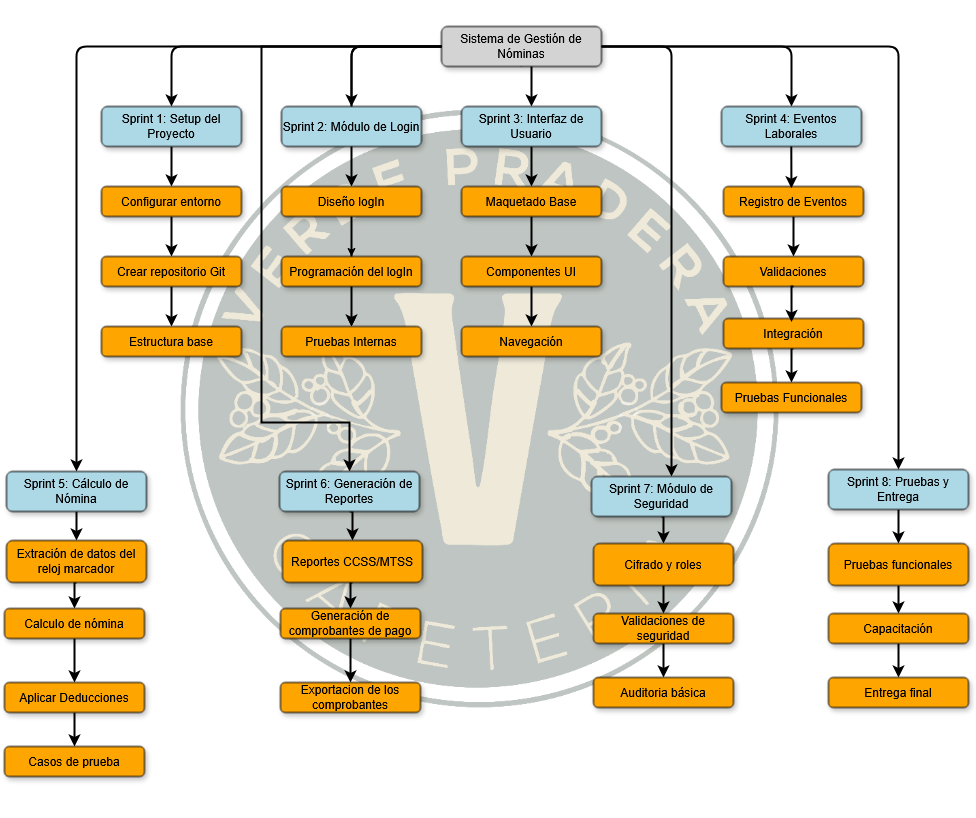
\includegraphics[width=1.0\textwidth]{media/EDT_VP-PLANILLAS.png}
	\caption{Estructura de Desglose del Trabajo del Proyecto (EDT) basada en sprints}
	\label{fig:edt}
\end{figure}


\subsection*{Product Backlog}

Antes de desarrollar las historias de usuario, se construyó un \textbf{Product Backlog} con las funcionalidades principales del sistema. Este backlog funciona como una lista priorizada de los entregables que serán desarrollados a lo largo de los sprints definidos. Cada ítem representa una funcionalidad o módulo del sistema, estimado en complejidad y valor para el usuario final.

El backlog sirve como guía para la planificación iterativa del proyecto, y puede evolucionar conforme se obtenga retroalimentación durante las etapas de desarrollo.

\begin{itemize}
	\item Autenticación y control de acceso
	\item Registro de jornada laboral desde lector de huella
	\item Gestión de eventos laborales (vacaciones, incapacidades)
	\item Cálculo automático de nómina
	\item Generación de reportes institucionales
	\item Emisión de comprobantes de pago
	\item Módulo de administración de usuarios
	\item Seguridad y roles
	\item Capacitación y documentación
\end{itemize}

\subsection*{Historias de Usuario}

Las historias de usuario permiten capturar de manera sencilla y centrada en el usuario las funcionalidades esperadas del sistema de gestión de nóminas para Café y Vivero Verde Pradera. Estas historias han sido redactadas desde la perspectiva de los distintos tipos de usuarios del sistema (administradores, colaboradores y gerentes), con el fin de comprender sus necesidades, priorizar el desarrollo de funcionalidades y planificar el trabajo en sprints.

Cada historia incluye información clave como el usuario involucrado, la prioridad del requerimiento, el riesgo asociado, la iteración en que se desarrollará, la estimación de esfuerzo y una breve descripción del comportamiento esperado del sistema.

Estas historias se utilizarán como base para guiar el diseño, implementación y pruebas de cada funcionalidad a lo largo del desarrollo del proyecto.

\begin{table}[h]
	\centering
	\caption{Historia de Usuario HU-01}
	\begin{tabular}{|p{5cm}|p{9cm}|}
		\hline
		\textbf{Número:}                          & HU-01                           \\ \hline
		\textbf{Nombre:}                          & Gestión de usuarios del sistema \\ \hline
		\textbf{Usuario:}                         & Administrador                   \\ \hline
		\textbf{Modificación de Historia Número:} & Nueva                           \\ \hline
		\textbf{Prioridad en Negocio:}            & Alta                            \\ \hline
		\textbf{Riesgo en Desarrollo:}            & Medio                           \\ \hline
		\textbf{Iteración Asignada:}              & Sprint 2: Módulo de Login       \\ \hline
		\textbf{Puntos Estimados:}                & 5                               \\ \hline
		\textbf{Puntos Reales:}                   & --                              \\ \hline
		\textbf{Descripción:}                     &
		El sistema permitirá al administrador realizar operaciones CRUD (Crear, Leer, Actualizar, Eliminar) sobre los usuarios registrados.
		El administrador podrá:
		\begin{itemize}
			\item Crear nuevos usuarios ingresando nombre, correo y rol.
			\item Consultar la lista de usuarios registrados.
			\item Editar los datos de un usuario existente (excepto el ID).
			\item Eliminar usuarios en caso de salida de personal.
		\end{itemize}
		Las acciones estarán disponibles únicamente para usuarios con rol de Administrador autenticado. Todas las operaciones deben registrar trazabilidad en la bitácora del sistema.
		\\ \hline
		\textbf{Observaciones:}                   &
		El correo ingresado debe ser validado en formato y unicidad. No se podrá eliminar al usuario con sesión activa.
		Solo se permite modificar el rol o correo si el usuario está inactivo.
		El sistema debe confirmar cada operación antes de ejecutarla.
		\\ \hline
	\end{tabular}
\end{table}


\begin{table}[h]
	\centering
	\caption{Historia de Usuario HU-02}
	\begin{tabular}{|p{5cm}|p{9cm}|}
		\hline
		\textbf{Número:}                          & HU-02                                   \\ \hline
		\textbf{Nombre:}                          & Gestión de roles de usuario             \\ \hline
		\textbf{Usuario:}                         & Administrador                           \\ \hline
		\textbf{Modificación de Historia Número:} & Nueva                                   \\ \hline
		\textbf{Prioridad en Negocio:}            & Alta                                    \\ \hline
		\textbf{Riesgo en Desarrollo:}            & Bajo                                    \\ \hline
		\textbf{Iteración Asignada:}              & Sprint 3: Módulo de Interfaz de Usuario \\ \hline
		\textbf{Puntos Estimados:}                & 5                                       \\ \hline
		\textbf{Puntos Reales:}                   & --                                      \\ \hline
		\textbf{Descripción:}                     &
		El sistema permitirá al administrador realizar operaciones CRUD sobre los roles asignados a los usuarios. Estas operaciones incluyen:
		\begin{itemize}
			\item \textbf{Crear:} Definir nuevos roles dentro del sistema si se requiere extender la funcionalidad futura.
			\item \textbf{Leer:} Consultar el rol asignado a cada usuario.
			\item \textbf{Actualizar:} Modificar el rol de un usuario existente.
			\item \textbf{Eliminar:} Eliminar roles obsoletos, siempre que no estén asignados a usuarios activos.
		\end{itemize}
		El administrador podrá ingresar a la sección de gestión de roles, seleccionar un usuario, visualizar los roles disponibles y asignar o modificar el rol correspondiente. El sistema guardará los cambios y mostrará una confirmación.
		\\ \hline
		\textbf{Observaciones:}                   &
		Cada usuario solo puede tener un rol activo a la vez.
		No se permitirá eliminar un rol si está actualmente asignado a uno o más usuarios.
		La acción de cambio de rol debe registrarse en la bitácora del sistema.
		La asignación de roles debe estar protegida por validación de permisos del administrador.
		\\ \hline
	\end{tabular}
\end{table}



\begin{table}[h]
	\centering
	\caption{Historia de Usuario HU-03}
	\begin{tabular}{|p{5cm}|p{9cm}|}
		\hline
		\textbf{Número:}                          & HU-03                                          \\ \hline
		\textbf{Nombre:}                          & Visualización y entrega del historial de pagos \\ \hline
		\textbf{Usuario:}                         & Colaborador                                    \\ \hline
		\textbf{Modificación de Historia Número:} & Nueva                                          \\ \hline
		\textbf{Prioridad en Negocio:}            & Media                                          \\ \hline
		\textbf{Riesgo en Desarrollo:}            & Bajo                                           \\ \hline
		\textbf{Iteración Asignada:}              & Sprint 5: Cálculo de Nóminas                   \\ \hline
		\textbf{Puntos Estimados:}                & 5                                              \\ \hline
		\textbf{Puntos Reales:}                   & --                                             \\ \hline
		\textbf{Descripción:}                     &
		El sistema permitirá a los colaboradores consultar su historial de pagos desde su perfil. Cada entrada mostrará la fecha del pago, el monto neto recibido, y un enlace para visualizar o descargar el comprobante oficial correspondiente.

		Además, por cumplimiento legal, el sistema enviará automáticamente una copia del comprobante de pago al correo electrónico registrado de cada colaborador al momento de realizar el cálculo de nómina.

		Las operaciones involucradas en este módulo consideran:
		\begin{itemize}
			\item \textbf{Crear:} El sistema generará un nuevo registro de pago cada vez que se procese una nómina.
			\item \textbf{Leer:} Los colaboradores pueden consultar su historial filtrando por rango de fechas.
			\item \textbf{Actualizar:} No aplica para el colaborador. Solo los administradores pueden rectificar datos desde el módulo de nómina.
			\item \textbf{Eliminar:} Los registros no podrán ser eliminados por los usuarios. Solo se podrán ocultar si hay rectificación con auditoría.
		\end{itemize}
		\\ \hline
		\textbf{Observaciones:}                   &
		Se debe asegurar la confidencialidad de los datos financieros mediante autenticación de usuario y cifrado de información. El comprobante de pago deberá cumplir con los requisitos legales del Ministerio de Trabajo y será enviado automáticamente al correo del colaborador una vez generado.
		\\ \hline
	\end{tabular}
\end{table}



\begin{table}[h]
	\centering
	\caption{Historia de Usuario HU-04}
	\begin{tabular}{|p{5cm}|p{9cm}|}
		\hline
		\textbf{Número:}                          & HU-04                                      \\ \hline
		\textbf{Nombre:}                          & Generación y gestión de reportes de nómina \\ \hline
		\textbf{Usuario:}                         & Gerente                                    \\ \hline
		\textbf{Modificación de Historia Número:} & Nueva                                      \\ \hline
		\textbf{Prioridad en Negocio:}            & Alta                                       \\ \hline
		\textbf{Riesgo en Desarrollo:}            & Alto                                       \\ \hline
		\textbf{Iteración Asignada:}              & Sprint 6: Generación de Reportes           \\ \hline
		\textbf{Puntos Estimados:}                & 5                                          \\ \hline
		\textbf{Puntos Reales:}                   & --                                         \\ \hline
		\textbf{Descripción:}                     &
		El sistema permitirá al gerente generar, visualizar y gestionar reportes de nómina. Desde el módulo correspondiente, el usuario podrá seleccionar el mes deseado y obtener un archivo PDF que incluya detalles de salarios brutos, deducciones, aportes patronales y salario neto total.

		Las operaciones CRUD asociadas a esta historia son:
		\begin{itemize}
			\item \textbf{Crear:} Generación de un nuevo reporte mensual al cierre de la nómina.
			\item \textbf{Leer:} Consultar reportes anteriores, filtrados por mes o año.
			\item \textbf{Actualizar:} Regenerar un reporte si se realizaron ajustes a la nómina.
			\item \textbf{Eliminar:} Borrar reportes bajo condiciones de auditoría (solo si no han sido firmados o validados).
		\end{itemize}
		Todos los reportes deberán conservar trazabilidad en la bitácora del sistema y permitir exportación a PDF.
		\\ \hline
		\textbf{Observaciones:}                   &
		Esta funcionalidad estará restringida exclusivamente a usuarios con rol de Gerente. El sistema debe validar la autenticación y el rol activo antes de permitir acceso. Todos los archivos generados deberán protegerse mediante encriptación y almacenamiento seguro.
		\\ \hline
	\end{tabular}
\end{table}

\begin{table}[h]
	\centering
	\caption{Historia de Usuario HU-05}
	\begin{tabular}{|p{5cm}|p{9cm}|}
		\hline
		\textbf{Número:}                          & HU-05                                                                                                                                                                                                \\ \hline
		\textbf{Nombre:}                          & Registro de llegada y salida de jornada laboral                                                                                                                                                      \\ \hline
		\textbf{Usuario:}                         & Colaborador                                                                                                                                                                                          \\ \hline
		\textbf{Modificación de Historia Número:} & Nueva                                                                                                                                                                                                \\ \hline
		\textbf{Prioridad en Negocio:}            & Alta                                                                                                                                                                                                 \\ \hline
		\textbf{Riesgo en Desarrollo:}            & Medio                                                                                                                                                                                                \\ \hline
		\textbf{Iteración Asignada:}              & Sprint 4: Eventos Laborales                                                                                                                                                                          \\ \hline
		\textbf{Puntos Estimados:}                & 5                                                                                                                                                                                                    \\ \hline
		\textbf{Puntos Reales:}                   & --                                                                                                                                                                                                   \\ \hline
		\textbf{Descripción:}                     &
		El colaborador registrará su ingreso y salida mediante un lector de huella o interfaz web. El sistema almacenará la hora exacta, la fecha y el ID del usuario, generando un historial de asistencia consultable por los administradores.

		\textbf{CRUD:}
		\begin{itemize}
			\item \textbf{Crear:} Registro automático del ingreso y salida al marcar asistencia.
			\item \textbf{Leer:} Consulta de historial por parte de administradores o el mismo colaborador.
			\item \textbf{Actualizar:} Solo en casos excepcionales por parte de administradores (con justificación).
			\item \textbf{Eliminar:} No permitido. Solo se puede anular con bitácora de rectificación.
		\end{itemize}
		\\ \hline
		\textbf{Observaciones:}                   & Se debe garantizar que el colaborador no pueda marcar por otro. La validación se puede hacer mediante huella digital o credenciales únicas. Toda modificación requiere justificación administrativa.
		\\ \hline
	\end{tabular}
\end{table}


\begin{table}[h]
	\centering
	\caption{Historia de Usuario HU-06}
	\begin{tabular}{|p{5cm}|p{9cm}|}
		\hline
		\textbf{Número:}                          & HU-06                                                                                                                               \\ \hline
		\textbf{Nombre:}                          & Generar documentación oficial para instituciones                                                                                    \\ \hline
		\textbf{Usuario:}                         & Gerente / Contabilidad                                                                                                              \\ \hline
		\textbf{Modificación de Historia Número:} & Nueva                                                                                                                               \\ \hline
		\textbf{Prioridad en Negocio:}            & Alta                                                                                                                                \\ \hline
		\textbf{Riesgo en Desarrollo:}            & Medio                                                                                                                               \\ \hline
		\textbf{Iteración Asignada:}              & Sprint 6: Generación de Reportes                                                                                                    \\ \hline
		\textbf{Puntos Estimados:}                & 5                                                                                                                                   \\ \hline
		\textbf{Puntos Reales:}                   & --                                                                                                                                  \\ \hline
		\textbf{Descripción:}                     &
		El sistema permitirá generar reportes mensuales en formatos requeridos por entidades como la CCSS, el Ministerio de Trabajo y el área de Contabilidad. Los datos incluirán horas trabajadas, deducciones, aportes patronales, y salarios netos.

		\textbf{CRUD:}
		\begin{itemize}
			\item \textbf{Crear:} Generación automática de reportes por mes o quincena.
			\item \textbf{Leer:} Consultar reportes anteriores.
			\item \textbf{Actualizar:} Regenerar reportes si hay ajustes contables.
			\item \textbf{Eliminar:} No permitido. Se puede anular con una versión rectificada.
		\end{itemize}
		\\ \hline
		\textbf{Observaciones:}                   & Los reportes deberán tener firma digital o código de validación. El acceso debe estar restringido por rol y registrado en bitácora.
		\\ \hline
	\end{tabular}
\end{table}


\begin{table}[h]
	\centering
	\caption{Historia de Usuario HU-07}
	\begin{tabular}{|p{5cm}|p{9cm}|}
		\hline
		\textbf{Número:}                          & HU-07                                                                                                                                           \\ \hline
		\textbf{Nombre:}                          & Registro y gestión de empleados                                                                                                                 \\ \hline
		\textbf{Usuario:}                         & Administrador                                                                                                                                   \\ \hline
		\textbf{Modificación de Historia Número:} & Nueva                                                                                                                                           \\ \hline
		\textbf{Prioridad en Negocio:}            & Alta                                                                                                                                            \\ \hline
		\textbf{Riesgo en Desarrollo:}            & Medio                                                                                                                                           \\ \hline
		\textbf{Iteración Asignada:}              & Sprint 1: Setup del Proyecto                                                                                                                    \\ \hline
		\textbf{Puntos Estimados:}                & 5                                                                                                                                               \\ \hline
		\textbf{Puntos Reales:}                   & --                                                                                                                                              \\ \hline
		\textbf{Descripción:}                     &
		El administrador podrá registrar, consultar, editar o desactivar a los colaboradores del sistema. Cada empleado tendrá asociado su nombre completo, número de cédula, correo, puesto y fecha de ingreso.

		\textbf{CRUD:}
		\begin{itemize}
			\item \textbf{Crear:} Registro de un nuevo colaborador con sus datos básicos.
			\item \textbf{Leer:} Consulta de empleados activos e inactivos.
			\item \textbf{Actualizar:} Modificación de datos personales o laborales.
			\item \textbf{Eliminar:} No aplica. Solo se desactiva al empleado manteniendo el historial.
		\end{itemize}
		\\ \hline
		\textbf{Observaciones:}                   & El sistema debe validar que el correo y la cédula no se repitan. Solo administradores pueden gestionar empleados. Toda acción queda registrada.
		\\ \hline
	\end{tabular}
\end{table}


\clearpage


\subsection*{Especificación de Requerimientos de Software (SRS)}
\subsection*{Introducción}
Esta Especificación de Requerimientos de Software (SRS) describe los
requerimientos funcionales y no funcionales del sistema web de gestión de nómina
para la empresa Café y Vivero Verde Pradera. Está dirigida al equipo de desarrollo,
usuarios finales, patrocinadores del proyecto y cualquier persona involucrada en la
validación y verificación del sistema.

\subsubsection*{Propósito}
El sistema gestionará de forma automatizada el cálculo de nómina, eventos laborales,
reportes institucionales y seguridad de datos del personal. Será accesible mediante
navegador web, con controles de acceso para usuarios autorizados. No incluirá
funcionalidades de facturación, contabilidad general o inventario.

\subsubsection*{Alcance}

El sistema gestionará de forma automatizada el cálculo de nómina,
eventos laborales, reportes institucionales y seguridad de datos del
personal. Será accesible mediante navegador web, con controles de acceso
para usuarios autorizados. No incluirá funcionalidades de facturación,
contabilidad general o inventario.

\subsubsection*{Definiciones, siglas y abreviaturas}

\begin{itemize}
	\item \textbf{SRS:} \textit{Software Requirements Specification}.
	\item \textbf{CCSS:} \textit{Caja Costarricense del Seguro Social}.
	\item \textbf{MTSS:} \textit{Ministerio de Trabajo y Seguridad Social}.
	\item \textbf{Nómina:} Proceso de cálculo de salarios y deducciones laborales.
	\item \textbf{Scrum:} Marco de trabajo ágil para gestión de proyectos.
	\item \textbf{VPG\_:} Prefijo usado para nombrar tablas en la base de datos.
\end{itemize}

\subsubsection*{Referencias}

\begin{itemize}
	\item \textbf{TFM del proyecto:} “Sistema de Gestión de Nóminas para Café y Vivero Verde Pradera”. Universidad Nacional, Sede Regional Brunca.

	\item \textbf{Scrum Guide (2020):} Guía oficial de la metodología Scrum por Ken Schwaber y Jeff Sutherland.

	\item \textbf{Normativa de la CCSS:} Requisitos para la generación y entrega de reportes laborales a la Caja Costarricense del Seguro Social.

	\item \textbf{Ministerio de Trabajo y Seguridad Social de Costa Rica:} Lineamientos legales sobre remuneraciones, horarios laborales, licencias y documentación obligatoria relacionada con la gestión de personal.
\end{itemize}


\subsubsection*{Visión general del documento}
\begin{itemize}
	\item \textbf{Sección 2:} Proporciona una descripción general del sistema, incluyendo su perspectiva, funciones principales, usuarios y restricciones de diseño.

	\item \textbf{Sección 3:} Detalla los requerimientos específicos, incluyendo casos de uso del sistema y requerimientos suplementarios.

	\item \textbf{Sección 4:} Describe los requerimientos de documentación que acompañarán al sistema.

\end{itemize}

\subsection*{Descripción General}

Esta sección presenta una visión global del sistema de gestión de nóminas para
Café y Vivero Verde Pradera. Aquí se describen los factores generales que influyen en
el desarrollo del software, tales como el entorno operativo, los usuarios involucrados,
las funciones principales y las restricciones de diseño. Aunque esta sección no entra en
detalle sobre los requerimientos específicos, sienta las bases conceptuales y técnicas que
guían el resto del documento.

\subsubsection*{Perspectiva del producto}

El sistema de gestión de nóminas es una aplicación web que funcionará como un
producto independiente, aunque podría integrarse a futuro con otros sistemas de gestión
empresarial. Su diseño sigue el modelo de n capas , con acceso controlado mediante
credenciales de usuario. El sistema será accesible mediante navegadores modernos desde
cualquier ubicación con conexión a internet.

\subsubsection*{Interfaces de usuario}

\begin{itemize}
	\item Pantalla de inicio de sesión
	\item Panel principal con resumen de información
	\item Módulo de gestión de empleados
	\item Módulo de cálculo y visualización de nómina
	\item Módulo de eventos laborales (vacaciones, incapacidades, permisos)
	\item Módulo de reportes (PDF/Excel)
	\item Módulo de configuración del sistema
	\item Mensajes de validación y error amigables
\end{itemize}

\subsubsection*{Interfaces de Hardware}

\begin{itemize}
	\item El sistema requerirá interacción con impresoras para generar documentos
	      físicos como comprobantes de pago, reportes y formularios.

	\item Se requerirá la integración con un reloj marcador, que permitirá subir
	      automáticamente los registros de entrada y salida del personal al sistema.
	      Estos datos serán utilizados para el cálculo de la nómina, especialmente en
	      el control de jornadas laborales, horas extra e inasistencias.

	\item La integración podrá realizarse mediante archivos de exportación (CSV, Excel)
	      generados por el reloj marcador, o mediante una conexión directa a través de API,
	      dependiendo del modelo del dispositivo.

\end{itemize}


\subsubsection*{Interfaces con software}

\begin{itemize}
	\item \textbf{Navegadores compatibles:} Chrome, Firefox, Microsoft Edge.

	\item \textbf{Base de datos:} Se utilizará una base de datos relacional, con preferencia por PostgreSQL o SQL Server, según disponibilidad y requisitos del entorno de producción.

	\item \textbf{Frameworks y tecnologías principales:}
	      \begin{itemize}
		      \item \textbf{Frontend:} Next.js con TypeScript, para el desarrollo de una aplicación web moderna, escalable y optimizada.
		      \item \textbf{Backend:} Node.js con Express.js, para construir una API REST robusta y eficiente que conecte con la base de datos y gestione la lógica de negocio.
	      \end{itemize}

	\item \textbf{Librerías complementarias:}
	      \begin{itemize}
		      \item Generación de reportes en PDF (por ejemplo, PDFKit o jsPDF).
		      \item Prisma ORM para la gestión de base de datos.
		      \item Librerías de validación, autenticación y control de acceso.
	      \end{itemize}
\end{itemize}


\subsubsection*{Interfaces de comunicación}

\begin{itemize}
	\item HTTP/HTTPS como protocolo de comunicación principal.
	\item APIs REST para el intercambio de datos entre frontend y backend.
	\item Encriptación SSL/TLS para comunicaciones seguras.
\end{itemize}

\subsubsection*{Restricciones de memoria}

El sistema está diseñado para operar eficientemente en servidores con un mínimo de:

\begin{itemize}
	\item Memoria RAM: 4GB
	\item Almacenamiento: 20GB
\end{itemize}

Los navegadores cliente deben tener al menos 1GB de RAM disponible.

\subsubsection*{Requerimientos de adecuación al entorno}

\begin{itemize}
	\item El sistema se adapta a diferentes dispositivos (responsive), permitiendo su uso en computadoras, laptops y tablets.
	\item Idioma predeterminado: Español (Costa Rica)
	\item El servidor deberá estar configurado con zona horaria GMT-6.
\end{itemize}

\subsubsection*{Funciones del producto (Casos de uso de alto nivel)}

\begin{itemize}
	\item Autenticación de usuarios
	\item Gestión de datos de empleados
	\item Cálculo automático de nómina
	\item Registro de eventos laborales (vacaciones, incapacidades, etc.)
	\item Generación de reportes oficiales
	\item Visualización de comprobantes de pago
	\item Control de accesos y seguridad
	\item Capacitación y ayuda al usuario
\end{itemize}

\subsubsection*{Características de los usuarios}

\begin{itemize}
	\item \textbf{Administrador:} Usuario principal del sistema, con experiencia en gestión administrativa. Es responsable de registrar y mantener los datos del personal, roles, jornadas, eventos laborales, generar la nómina, administrar usuarios y emitir reportes oficiales. Tiene acceso total a todos los módulos del sistema, incluyendo la configuración de seguridad y la bitácora.

	\item \textbf{Colaborador (Empleado):} Usuario con acceso restringido. Puede consultar su información personal, visualizar y descargar su historial de pagos, y recibir los comprobantes por correo. No tiene acceso a la administración de nómina, ni puede modificar sus datos directamente.

	\item \textbf{Gerente:} Usuario con acceso a los reportes consolidados de nómina. Puede generar documentación institucional (para CCSS, MTSS, contabilidad), consultar datos agregados y validar información histórica. No tiene permisos para editar nómina ni datos del personal.

	\item \textbf{Contabilidad (opcional):} Usuario con acceso exclusivo a los módulos de exportación de datos contables y reportes oficiales. Puede descargar formatos estandarizados y generar documentación legal.
\end{itemize}

\subsubsection*{Restricciones de diseño}

\begin{itemize}
	\item \textbf{Lenguaje backend:} TypeScript utilizando Node.js y Express.js como framework principal para el desarrollo de la API.
	\item \textbf{Lenguaje frontend:} Next.js con TypeScript, que ofrece funcionalidades modernas como renderizado híbrido (SSR/SSG) y excelente integración con React y Tailwind CSS para el diseño visual.
	\item \textbf{Base de datos:} PostgreSQL como base preferente por su robustez y escalabilidad, aunque puede considerarse SQL Server según la infraestructura del cliente.
	\item \textbf{ORM:} Prisma será utilizado como herramienta de mapeo objeto-relacional para facilitar la interacción entre la base de datos y el backend.
	\item \textbf{Arquitectura:} Modelo cliente-servidor basado en APIs REST, con separación clara entre frontend (interfaz de usuario) y backend (lógica de negocio y persistencia).
	\item \textbf{Control de versiones:} Git, utilizando GitHub como plataforma central para la gestión del código fuente, seguimiento de cambios y colaboración mediante Pull Requests.
	\item \textbf{Estandarización en base de datos:} Se utilizará un esquema consistente de nomenclatura, donde las tablas comienzan con el prefijo VPG\_ seguido del nombre en mayúsculas, y las columnas en minúsculas con guion bajo.
\end{itemize}

\subsubsection*{Restricción de diseño 1}

\textbf{Uso obligatorio de Next.js con TypeScript como framework de desarrollo frontend.}
El sistema debe ser desarrollado utilizando el framework Next.js con TypeScript como lenguaje principal, por su capacidad de renderizado híbrido, manejo eficiente del enrutamiento y escalabilidad. Esta decisión es clave para mantener un entorno moderno, seguro y compatible con estándares actuales de desarrollo web.

\subsubsection*{Restricción de diseño 2}

\textbf{Backend implementado en Express.js con Node.js y TypeScript.}
La lógica de negocio del sistema debe ser implementada mediante una API RESTful utilizando Express.js sobre Node.js, con escritura en TypeScript para mejorar la robustez del código. Esta tecnología ha sido elegida por su ligereza, flexibilidad, comunidad activa y compatibilidad con herramientas modernas de desarrollo.

\subsubsection*{Restricción de diseño 3}

\textbf{Uso de PostgreSQL como base de datos principal.}
La base de datos del sistema será implementada en PostgreSQL, salvo que se requiera específicamente el uso de SQL Server por condiciones de infraestructura del cliente. PostgreSQL fue seleccionado por su alto rendimiento, seguridad, soporte para transacciones ACID y amplia compatibilidad con herramientas ORM modernas.

\subsubsection*{Restricción de diseño 4}

\textbf{ORM Prisma para gestión de la base de datos.}
Se utilizará Prisma como herramienta de mapeo objeto-relacional (ORM) para interactuar con la base de datos. Prisma proporciona tipado fuerte, migraciones estructuradas y una experiencia de desarrollo alineada con TypeScript, lo que facilita la validación y mantenimiento del sistema.

\subsubsection*{Restricción de diseño 5}

\textbf{Modelo de arquitectura cliente-servidor basado en APIs REST.}
El sistema adoptará una arquitectura cliente-servidor, donde la interfaz de usuario (frontend) se comunica con el backend a través de una API REST. Esta separación garantiza una mejor escalabilidad, facilita el mantenimiento del código y permite una posible integración futura con otros sistemas.

\subsubsection*{Restricción de diseño 6}

\textbf{Control de versiones obligatorio con Git y repositorio en GitHub.}
Todo el código fuente del sistema será gestionado mediante Git, con uso obligatorio del repositorio GitHub. Se seguirán buenas prácticas como el uso de ramas (main, develop, feature/*), mensajes de commit con prefijos ([FEATURE], [FIXED], [BUG], etc.) y revisiones por medio de pull requests para evitar conflictos y mantener calidad de código.

\subsubsection*{Restricción de diseño 7}

\textbf{Nomenclatura de base de datos estandarizada.}
Las tablas en la base de datos deberán seguir el prefijo VPG\_ en mayúsculas, mientras que los campos se escribirán en minúsculas con guion bajo (snake\_case). Las claves foráneas seguirán el formato VPG\_TABLA1\_TABLA2\_FK. Esto garantiza consistencia, claridad y facilita la lectura del modelo de datos.

\subsubsection*{Supuestos y dependencias}

\begin{itemize}
	\item Se asume que los usuarios tienen conocimientos básicos en el uso de sistemas web.
	\item Se espera que la empresa mantenga infraestructura básica (conectividad, energía eléctrica).
	\item Cualquier cambio en la legislación laboral podría requerir ajustes al sistema.
\end{itemize}


\subsection*{Requerimientos del Sistema}

Esta sección detalla los requerimientos funcionales y no funcionales del sistema
de gestión de nóminas para Café y Vivero Verde Pradera. Los requerimientos se han
organizado utilizando el modelo de casos de uso para representar las funcionalidades
principales, así como especificaciones suplementarias que cubren aspectos como rendimiento,
seguridad, usabilidad y documentación.

La información aquí contenida proporciona el nivel de detalle necesario para que el
equipo de desarrollo diseñe e implemente el sistema, y para que los encargados de calidad
validen su cumplimiento mediante pruebas.

\subsubsection*{Modelo de Caso de Uso de Negocio}

El modelo de negocio se centra en optimizar la gestión de nóminas del personal de la empresa Café y Vivero Verde Pradera. A continuación, se enumeran los principales procesos, definidos con base en las historias de usuario priorizadas:

\begin{itemize}
	\item Ingreso al sistema (autenticación de usuarios)
	\item Registro y administración de empleados
	\item Asignación y gestión de roles de usuario
	\item Registro de jornada laboral (llegada y salida)
	\item Registro y administración de eventos laborales (vacaciones, incapacidades, permisos)
	\item Cálculo automático de salarios y deducciones
	\item Generación de reportes oficiales (CCSS, MTSS, contabilidad)
	\item Emisión de comprobantes de pago a colaboradores
	\item Configuración de parámetros del sistema (pendiente de historia funcional)
\end{itemize}

Estos procesos serán representados como Casos de Uso en el sistema de información.

\subsubsection*{Modelo de Caso de Uso de Sistema}

\begin{table}[h]
	\centering
	\caption{Modelo de Casos de Uso del Sistema}
	\begin{tabular}{|c|p{6cm}|p{5cm}|}
		\hline
		\textbf{Código} & \textbf{Nombre de Caso de uso}    & \textbf{Actor Principal} \\ \hline
		CU01            & Iniciar Sesión                    & Usuario autorizado       \\ \hline
		CU02            & Registrar empleado                & Administrador            \\ \hline
		CU03            & Editar información de empleado    & Administrador            \\ \hline
		CU04            & Registrar evento laboral          & Administrador            \\ \hline
		CU05            & Calcular nómina                   & Administrador            \\ \hline
		CU06            & Generar reporte para la CCSS      & Administrador            \\ \hline
		CU07            & Consultar comprobante de pago     & Administrador            \\ \hline
		CU08            & Configurar parámetros del sistema & Administrador            \\ \hline
	\end{tabular}
\end{table}

\clearpage

\subsubsection*{Especificación de Caso de Uso: CU01 - Iniciar sesión}

\begin{table}[h]
	\centering
	\caption{Especificación de Caso de Uso CU01 - Iniciar sesión}
	\begin{tabular}{|p{5cm}|p{9cm}|}
		\hline
		\textbf{Especificación de Caso de Uso} & CU01 - Iniciar sesión \\ \hline
		\textbf{Versión}                       & 1.0                   \\ \hline
		\textbf{CU de Negocio}                 & Iniciar sesión        \\ \hline
		\textbf{Fecha}                         & 10/04/2025            \\ \hline
		\textbf{Código del Caso de Uso}        & CU01                  \\ \hline
	\end{tabular}
\end{table}

\subsubsection*{Descripción}
Este caso de uso permite a los usuarios autorizados acceder al sistema mediante autenticación.

\subsubsection*{Precondiciones}
\begin{itemize}
	\item El usuario debe estar registrado previamente en el sistema.
	\item El navegador debe tener conexión activa a internet.
	\item El sistema debe estar disponible.
\end{itemize}

\subsubsection*{Poscondiciones}
\begin{itemize}
	\item El usuario accede al sistema con los permisos correspondientes.
	\item Se registra la hora de acceso en el historial.
\end{itemize}

\subsubsection*{Referencias}
CU02

\clearpage

\subsubsection*{Flujo de Eventos}
\begin{table}[h]
	\centering
	\caption{Flujo principal de eventos}
	\begin{tabular}{|p{7cm}|p{7cm}|}
		\hline
		\textbf{Acción del actor}                     & \textbf{Respuesta del sistema}                              \\ \hline
		El usuario abre la página de inicio de sesión & El sistema muestra el formulario de autenticación           \\ \hline
		El usuario ingresa sus credenciales           & El sistema valida las credenciales                          \\ \hline
		El usuario hace clic en 'Iniciar sesión'      & El sistema concede acceso si las credenciales son correctas \\ \hline
	\end{tabular}
\end{table}

\subsubsection*{Flujos alternos}
\begin{table}[h]
	\centering
	\caption{Flujos alternos}
	\begin{tabular}{|p{7cm}|p{7cm}|}
		\hline
		\textbf{Acción del actor}                     & \textbf{Respuesta del sistema}                                       \\ \hline
		El usuario deja campos vacíos                 & El sistema muestra un mensaje de error indicando campos obligatorios \\ \hline
		El usuario introduce credenciales incorrectas & El sistema muestra 'Credenciales inválidas'                          \\ \hline
	\end{tabular}
\end{table}

\subsubsection*{Excepciones}
\begin{table}[h]
	\centering
	\caption{Excepciones del caso de uso CU01}
	\begin{tabular}{|p{4cm}|p{6cm}|p{6cm}|}
		\hline
		\textbf{Código Excepción} & \textbf{Evento}      & \textbf{Excepción}                        \\ \hline
		E001                      & Servidor no responde & Mostrar mensaje: 'Servicio no disponible' \\ \hline
		E002                      & Usuario bloqueado    & Mostrar advertencia y denegar acceso      \\ \hline
	\end{tabular}
\end{table}

\subsubsection*{Estado}
En definición

\subsubsection*{Especificación de Caso de Uso: CU02 - Registrar empleado}

\begin{table}[h]
	\centering
	\caption{Especificación de Caso de Uso CU02 - Registrar empleado}
	\begin{tabular}{|p{5cm}|p{9cm}|}
		\hline
		\textbf{Especificación de Caso de Uso} & CU02 - Registrar empleado \\ \hline
		\textbf{Versión}                       & 1.0                       \\ \hline
		\textbf{CU de Negocio}                 & Registro de empleados     \\ \hline
		\textbf{Fecha}                         & 10/04/2025                \\ \hline
		\textbf{Código del Caso de Uso}        & CU02                      \\ \hline
	\end{tabular}
\end{table}

\subsubsection*{Descripción}
Este caso de uso permite al administrador registrar nuevos empleados en el sistema, ingresando datos personales, laborales y de contacto. Esta información se usará en procesos de nómina, reportes y control administrativo.

\subsubsection*{Precondiciones}
\begin{itemize}
	\item El usuario debe haber iniciado sesión como administrador.
	\item El sistema debe estar conectado a la base de datos.
	\item El formulario de registro debe estar disponible.
\end{itemize}

\subsubsection*{Poscondiciones}
\begin{itemize}
	\item El nuevo empleado queda registrado correctamente en la base de datos.
	\item La información se encuentra disponible para ser consultada y utilizada por otros módulos.
\end{itemize}

\subsubsection*{Referencias}
CU01, CU03, CU05

\clearpage

\subsubsection*{Flujo de Eventos}
\begin{table}[h]
	\centering
	\caption{Flujo principal de eventos}
	\begin{tabular}{|p{7cm}|p{7cm}|}
		\hline
		\textbf{Acción del actor}                        & \textbf{Respuesta del sistema}                       \\ \hline
		El administrador selecciona “Registrar empleado” & El sistema muestra el formulario de registro         \\ \hline
		El administrador llena los campos requeridos     & El sistema valida los datos ingresados               \\ \hline
		El administrador hace clic en “Guardar”          & El sistema almacena los datos y confirma el registro \\ \hline
	\end{tabular}
\end{table}

\subsubsection*{Flujos alternos}
\begin{table}[h]
	\centering
	\caption{Flujos alternos}
	\begin{tabular}{|p{7cm}|p{7cm}|}
		\hline
		\textbf{Acción del actor}                               & \textbf{Respuesta del sistema}                                     \\ \hline
		El administrador deja campos obligatorios sin completar & El sistema muestra mensaje de error y resalta los campos faltantes \\ \hline
		El administrador ingresa una cédula ya registrada       & El sistema muestra advertencia: "Empleado ya registrado"           \\ \hline
	\end{tabular}
\end{table}

\subsubsection*{Excepciones}
\begin{table}[h]
	\centering
	\caption{Excepciones del caso de uso CU02}
	\begin{tabular}{|p{3cm}|p{5cm}|p{5cm}|}
		\hline
		\textbf{Código Excepción} & \textbf{Evento}                        & \textbf{Excepción}                                       \\ \hline
		E001                      & Fallo de conexión con la base de datos & Mostrar mensaje: 'No se pudo guardar, intente más tarde' \\ \hline
		E002                      & Formato incorrecto de algún dato       & Mostrar advertencia y evitar el guardado                 \\ \hline
	\end{tabular}
\end{table}

\newpage

\subsubsection*{Estado}
En definición

\subsubsection*{Especificación de Caso de Uso: CU03 - Editar información de empleado}

\begin{table}[h]
	\centering
	\caption{Especificación de Caso de Uso CU03 - Editar información de empleado}
	\begin{tabular}{|p{5cm}|p{9cm}|}
		\hline
		\textbf{Especificación de Caso de Uso} & CU03 - Editar información de empleado \\ \hline
		\textbf{Versión}                       & 1.0                                   \\ \hline
		\textbf{CU de Negocio}                 & Registro de empleados                 \\ \hline
		\textbf{Fecha}                         & 10/04/2025                            \\ \hline
		\textbf{Código del Caso de Uso}        & CU03                                  \\ \hline
	\end{tabular}
\end{table}

\subsubsection*{Descripción}
Este caso de uso permite al administrador modificar los datos personales o laborales de un empleado previamente registrado. Las modificaciones se reflejan en los procesos de cálculo de nómina, reportes y control administrativo.

\subsubsection*{Precondiciones}
\begin{itemize}
	\item El usuario debe haber iniciado sesión como administrador.
	\item Debe existir al menos un empleado registrado en el sistema.
	\item El sistema debe estar conectado a la base de datos.
\end{itemize}

\subsubsection*{Poscondiciones}
\begin{itemize}
	\item Los datos del empleado quedan actualizados en el sistema.
	\item Las nuevas configuraciones impactan en cálculos y reportes futuros.
\end{itemize}

\subsubsection*{Referencias}
CU01, CU02, CU05

\clearpage

\subsubsection*{Flujo de Eventos}
\begin{table}[h]
	\centering
	\caption{Flujo principal de eventos}
	\begin{tabular}{|p{7cm}|p{7cm}|}
		\hline
		\textbf{Acción del actor}                       & \textbf{Respuesta del sistema}                            \\ \hline
		El administrador selecciona un empleado         & El sistema carga la información actual del empleado       \\ \hline
		El administrador modifica los campos deseados   & El sistema valida los datos modificados                   \\ \hline
		El administrador hace clic en “Guardar cambios” & El sistema actualiza los datos y muestra mensaje de éxito \\ \hline
	\end{tabular}
\end{table}

\subsubsection*{Flujos alternos}
\begin{table}[h]
	\centering
	\caption{Flujos alternos}
	\begin{tabular}{|p{7cm}|p{7cm}|}
		\hline
		\textbf{Acción del actor}                          & \textbf{Respuesta del sistema}                                  \\ \hline
		El administrador intenta guardar sin hacer cambios & El sistema muestra mensaje: "No se detectaron cambios"          \\ \hline
		El administrador deja campos obligatorios vacíos   & El sistema muestra advertencia y resalta los campos incompletos \\ \hline
	\end{tabular}
\end{table}

\subsubsection*{Excepciones}
\begin{table}[h]
	\centering
	\caption{Excepciones del caso de uso CU03}
	\begin{tabular}{|p{3cm}|p{5cm}|p{5cm}|}
		\hline
		\textbf{Código Excepción} & \textbf{Evento}                         & \textbf{Excepción}                                             \\ \hline
		E001                      & Fallo en la conexión a la base de datos & Mostrar mensaje: 'Error al guardar cambios, intente más tarde' \\ \hline
		E002                      & Formato inválido de datos               & Mostrar advertencia con campo específico                       \\ \hline
	\end{tabular}
\end{table}

\newpage

\subsubsection*{Estado}
En definición

\subsubsection*{Especificación de Caso de Uso: CU04 - Registrar evento laboral}

\begin{table}[h]
	\centering
	\caption{Especificación de Caso de Uso CU04 - Registrar evento laboral}
	\begin{tabular}{|p{5cm}|p{9cm}|}
		\hline
		\textbf{Especificación de Caso de Uso} & CU04 - Registrar evento laboral \\ \hline
		\textbf{Versión}                       & 1.0                             \\ \hline
		\textbf{CU de Negocio}                 & Registro de eventos laborales   \\ \hline
		\textbf{Fecha}                         & 10/04/2025                      \\ \hline
		\textbf{Código del Caso de Uso}        & CU04                            \\ \hline
	\end{tabular}
\end{table}

\subsubsection*{Descripción}
Este caso de uso permite al administrador registrar eventos laborales tales como vacaciones, incapacidades, permisos o ausencias de los empleados. Estos eventos afectan directamente el cálculo de la nómina.

\subsubsection*{Precondiciones}
\begin{itemize}
	\item El usuario debe haber iniciado sesión como administrador.
	\item Debe existir al menos un empleado registrado.
	\item El formulario de eventos laborales debe estar disponible.
\end{itemize}

\subsubsection*{Poscondiciones}
\begin{itemize}
	\item El evento queda registrado y asociado al empleado correspondiente.
	\item Los eventos se reflejan en el cálculo de la nómina.
\end{itemize}

\subsubsection*{Referencias}
CU01, CU02, CU05

\clearpage

\subsubsection*{Flujo de Eventos}
\begin{table}[h]
	\centering
	\caption{Flujo principal de eventos}
	\begin{tabular}{|p{7cm}|p{7cm}|}
		\hline
		\textbf{Acción del actor}                          & \textbf{Respuesta del sistema}                                \\ \hline
		El administrador selecciona un empleado            & El sistema carga el historial de eventos del empleado         \\ \hline
		El administrador escoge el tipo de evento y fechas & El sistema habilita los campos correspondientes               \\ \hline
		El administrador hace clic en “Registrar”          & El sistema guarda el evento y muestra mensaje de confirmación \\ \hline
	\end{tabular}
\end{table}

\subsubsection*{Flujos alternos}
\begin{table}[h]
	\centering
	\caption{Flujos alternos}
	\begin{tabular}{|p{7cm}|p{7cm}|}
		\hline
		\textbf{Acción del actor}                                         & \textbf{Respuesta del sistema}                                                     \\ \hline
		El administrador ingresa un rango de fechas inválido              & El sistema muestra advertencia: "Fecha de fin no puede ser menor que la de inicio" \\ \hline
		El administrador registra un evento duplicado en el mismo periodo & El sistema muestra mensaje: "Ya existe un evento en este periodo"                  \\ \hline
	\end{tabular}
\end{table}

\subsubsection*{Excepciones}
\begin{table}[h]
	\centering
	\caption{Excepciones del caso de uso CU04}
	\begin{tabular}{|p{3cm}|p{5cm}|p{5cm}|}
		\hline
		\textbf{Código Excepción} & \textbf{Evento}                   & \textbf{Excepción}                                               \\ \hline
		E001                      & Error al guardar en base de datos & Mostrar mensaje: 'No se pudo registrar el evento, intente luego' \\ \hline
		E002                      & Formato incorrecto de fecha       & Mostrar advertencia: 'Formato de fecha inválido'                 \\ \hline
	\end{tabular}
\end{table}

\newpage

\subsubsection*{Estado}
En definición

\subsection*{Especificación de Caso de Uso: CU05 - Calcular Nómina}

\begin{table}[h]
	\centering
	\caption{Especificación de Caso de Uso CU05 - Calcular nómina}
	\begin{tabular}{|p{5cm}|p{9cm}|}
		\hline
		\textbf{Especificación de Caso de Uso} & CU05 - Calcular nómina \\ \hline
		\textbf{Versión}                       & 1.0                    \\ \hline
		\textbf{CU de Negocio}                 & Cálculo de Salarios    \\ \hline
		\textbf{Fecha}                         & 08/04/2025             \\ \hline
		\textbf{Código del Caso de Uso}        & CU05                   \\ \hline
	\end{tabular}
\end{table}

\subsubsection*{Descripción}
Este caso de uso permite al administrador calcular la nómina mensual de todos los empleados, tomando en cuenta los eventos laborales registrados, salario base, deducciones obligatorias y horas trabajadas.

\subsubsection*{Precondiciones}
\begin{itemize}
	\item El usuario debe haber iniciado sesión.
	\item Deben existir empleados registrados en el sistema.
	\item Los eventos laborales deben estar actualizados.
\end{itemize}

\subsubsection*{Poscondiciones}
\begin{itemize}
	\item La nómina mensual queda registrada.
	\item Se generan comprobantes de pago individuales por empleado.
	\item Se habilita la generación de reportes para instituciones oficiales.
\end{itemize}

\subsubsection*{Referencias}
CU02, CU03, CU04

\clearpage

\subsubsection*{Flujo de Eventos}

\begin{table}[h]
	\centering
	\caption{Flujo principal de eventos}
	\begin{tabular}{|p{7cm}|p{7cm}|}
		\hline
		\textbf{Acción del actor}                            & \textbf{Respuesta del sistema}                              \\ \hline
		El usuario selecciona el mes y año a calcular        & El sistema carga los datos de empleados y eventos laborales \\ \hline
		El usuario confirma el cálculo                       & El sistema realiza el cálculo automático de salarios        \\ \hline
		El sistema muestra un resumen con los montos totales & Se habilita la opción de guardar y emitir comprobantes      \\ \hline
	\end{tabular}
\end{table}

\subsubsection*{Flujos alternos}

\begin{table}[h]
	\centering
	\caption{Flujos alternos}
	\begin{tabular}{|p{7cm}|p{7cm}|}
		\hline
		\textbf{Acción del actor}                                                   & \textbf{Respuesta del sistema}                                                                                                             \\ \hline
		El usuario selecciona un mes sin registros de eventos laborales             & El sistema muestra un aviso: "No se encontraron eventos laborales para este periodo" y permite continuar el cálculo solo con salarios base \\ \hline
		El usuario intenta calcular la nómina sin haber registrado nuevos empleados & El sistema muestra un mensaje de advertencia: "No hay empleados registrados para calcular nómina" y bloquea el proceso                     \\ \hline
		El usuario modifica manualmente un evento laboral antes del cálculo         & El sistema actualiza automáticamente los datos antes de procesar la nómina                                                                 \\ \hline
	\end{tabular}
\end{table}

\clearpage

\subsubsection*{Excepciones}

\begin{table}[h]
	\centering
	\caption{Excepciones del caso de uso CU05}
	\begin{tabular}{|p{4cm}|p{6cm}|p{6cm}|}
		\hline
		\textbf{Código Excepción} & \textbf{Evento}              & \textbf{Excepción}                     \\ \hline
		E001                      & No hay empleados activos     & Mostrar mensaje de error               \\ \hline
		E002                      & Datos incompletos en eventos & Mostrar advertencia y bloquear cálculo \\ \hline
	\end{tabular}
\end{table}

\subsubsection*{Estado}
En definición

\subsubsection*{Especificación de Caso de Uso: CU06 - Generar reporte para la CCSS}

\begin{table}[h]
	\centering
	\caption{Especificación de Caso de Uso CU06 - Generar reporte para la CCSS}
	\begin{tabular}{|p{5cm}|p{9cm}|}
		\hline
		\textbf{Especificación de Caso de Uso} & CU06 - Generar reporte para la CCSS \\ \hline
		\textbf{Versión}                       & 1.0                                 \\ \hline
		\textbf{CU de Negocio}                 & Generación de reportes oficiales    \\ \hline
		\textbf{Fecha}                         & 10/04/2025                          \\ \hline
		\textbf{Código del Caso de Uso}        & CU06                                \\ \hline
	\end{tabular}
\end{table}

\subsubsection*{Descripción}
Este caso de uso permite al administrador generar el reporte oficial de la nómina de un mes determinado, en el formato requerido por la Caja Costarricense del Seguro Social (CCSS). El reporte puede exportarse en PDF o Excel.

\subsubsection*{Precondiciones}
\begin{itemize}
	\item El usuario debe haber iniciado sesión como administrador.
	\item Debe existir una nómina calculada para el mes seleccionado.
	\item Los datos de empleados y deducciones deben estar actualizados.
\end{itemize}

\subsubsection*{Poscondiciones}
\begin{itemize}
	\item Se genera un archivo descargable con el reporte oficial.
	\item El evento queda registrado en la bitácora del sistema.
\end{itemize}

\subsubsection*{Referencias}
CU01, CU05, RS01

\subsubsection*{Flujo de Eventos}
\begin{table}[h]
	\centering
	\caption{Flujo principal de eventos}
	\begin{tabular}{|p{7cm}|p{7cm}|}
		\hline
		\textbf{Acción del actor}                          & \textbf{Respuesta del sistema}                                 \\ \hline
		El administrador selecciona “Generar reporte CCSS” & El sistema muestra el formulario de selección de mes y formato \\ \hline
		El administrador selecciona el mes y formato       & El sistema valida que exista nómina registrada para ese mes    \\ \hline
		El administrador hace clic en “Generar”            & El sistema genera el archivo y lo presenta para descarga       \\ \hline
	\end{tabular}
\end{table}

\subsubsection*{Flujos alternos}
\begin{table}[h]
	\centering
	\caption{Flujos alternos}
	\begin{tabular}{|p{7cm}|p{7cm}|}
		\hline
		\textbf{Acción del actor}                               & \textbf{Respuesta del sistema}                                             \\ \hline
		El administrador selecciona un mes sin nómina calculada & El sistema muestra advertencia: "No hay datos de nómina para este periodo" \\ \hline
		El administrador selecciona un formato no soportado     & El sistema muestra error: "Formato de exportación no disponible"           \\ \hline
	\end{tabular}
\end{table}

\newpage

\subsubsection*{Excepciones}
\begin{table}[h]
	\centering
	\caption{Excepciones del caso de uso CU06}
	\begin{tabular}{|p{3cm}|p{5cm}|p{5cm}|}
		\hline
		\textbf{Código Excepción} & \textbf{Evento}                    & \textbf{Excepción}                                                 \\ \hline
		E001                      & Error al generar el archivo        & Mostrar mensaje: 'No se pudo generar el archivo, intente de nuevo' \\ \hline
		E002                      & Plantilla de reporte no encontrada & Mostrar mensaje: 'Plantilla de reporte dañada o ausente'           \\ \hline
	\end{tabular}
\end{table}

\subsubsection*{Estado}
En definición


\subsubsection*{Especificación de Caso de Uso: CU07 - Consultar comprobante de pago}

\begin{table}[h]
	\centering
	\caption{Especificación de Caso de Uso CU07 - Consultar comprobante de pago}
	\begin{tabular}{|p{5cm}|p{9cm}|}
		\hline
		\textbf{Especificación de Caso de Uso} & CU07 - Consultar comprobante de pago \\ \hline
		\textbf{Versión}                       & 1.0                                  \\ \hline
		\textbf{CU de Negocio}                 & Emisión de comprobantes de pago      \\ \hline
		\textbf{Fecha}                         & 10/04/2025                           \\ \hline
		\textbf{Código del Caso de Uso}        & CU07                                 \\ \hline
	\end{tabular}
\end{table}

\subsubsection*{Descripción}
Este caso de uso permite tanto al administrador como al empleado (con acceso restringido) consultar los comprobantes de pago generados a partir de la nómina. El sistema permite visualizar e imprimir los comprobantes asociados a cada periodo.

\subsubsection*{Precondiciones}
\begin{itemize}
	\item El usuario debe haber iniciado sesión.
	\item Debe existir al menos un comprobante de pago generado.
	\item El sistema debe tener acceso a los archivos de comprobantes.
\end{itemize}

\subsubsection*{Poscondiciones}
\begin{itemize}
	\item El comprobante es visualizado correctamente por el usuario.
	\item El usuario puede descargar el comprobante en formato PDF.
\end{itemize}

\subsubsection*{Referencias}
CU01, CU05, CU06

\subsubsection*{Flujo de Eventos}
\begin{table}[h]
	\centering
	\caption{Flujo principal de eventos}
	\begin{tabular}{|p{7cm}|p{7cm}|}
		\hline
		\textbf{Acción del actor}                   & \textbf{Respuesta del sistema}                               \\ \hline
		El usuario accede al módulo “Comprobantes”  & El sistema muestra el listado de comprobantes disponibles    \\ \hline
		El usuario selecciona un mes                & El sistema carga el comprobante de pago correspondiente      \\ \hline
		El usuario hace clic en “Ver” o “Descargar” & El sistema presenta el comprobante en pantalla o lo descarga \\ \hline
	\end{tabular}
\end{table}

\subsubsection*{Flujos alternos}
\begin{table}[h]
	\centering
	\caption{Flujos alternos}
	\begin{tabular}{|p{7cm}|p{7cm}|}
		\hline
		\textbf{Acción del actor}                                    & \textbf{Respuesta del sistema}                                     \\ \hline
		El usuario selecciona un mes sin comprobante disponible      & El sistema muestra mensaje: "No hay comprobante para este periodo" \\ \hline
		El usuario intenta abrir un comprobante con error de formato & El sistema muestra mensaje: "Error al cargar el comprobante"       \\ \hline
	\end{tabular}
\end{table}

\subsubsection*{Excepciones}
\begin{table}[h]
	\centering
	\caption{Excepciones del caso de uso CU07}
	\begin{tabular}{|p{3cm}|p{5cm}|p{5cm}|}
		\hline
		\textbf{Código Excepción} & \textbf{Evento}       & \textbf{Excepción}                                           \\ \hline
		E001                      & Archivo no encontrado & Mostrar mensaje: 'Comprobante no disponible o fue eliminado' \\ \hline
		E002                      & Comprobante inválido  & Mostrar advertencia: 'El archivo no se puede visualizar'     \\ \hline
	\end{tabular}
\end{table}

\subsubsection*{Estado}
En definición

\subsubsection*{Especificación de Caso de Uso: CU08 - Configurar parámetros del sistema}

\begin{table}[h]
	\centering
	\caption{Especificación de Caso de Uso CU08 - Configurar parámetros del sistema}
	\begin{tabular}{|p{5cm}|p{9cm}|}
		\hline
		\textbf{Especificación de Caso de Uso} & CU08 - Configurar parámetros del sistema \\ \hline
		\textbf{Versión}                       & 1.0                                      \\ \hline
		\textbf{CU de Negocio}                 & Configuración del sistema                \\ \hline
		\textbf{Fecha}                         & 10/04/2025                               \\ \hline
		\textbf{Código del Caso de Uso}        & CU08                                     \\ \hline
	\end{tabular}
\end{table}

\subsubsection*{Descripción}
Este caso de uso permite al administrador modificar los parámetros globales del sistema, como tasas de deducción, salario mínimo, fechas de corte y opciones visuales. Estos parámetros afectan el comportamiento del sistema en diferentes módulos, incluyendo cálculo de nómina y reportes.

\subsubsection*{Precondiciones}
\begin{itemize}
	\item El usuario debe haber iniciado sesión como administrador.
	\item El sistema debe tener acceso a la base de datos de configuración.
	\item El formulario de configuración debe estar activo.
\end{itemize}

\subsubsection*{Poscondiciones}
\begin{itemize}
	\item Los parámetros quedan actualizados y se aplican al funcionamiento general del sistema.
	\item Las modificaciones se registran en la bitácora del sistema.
\end{itemize}

\subsubsection*{Referencias}
CU01, CU05, CU06

\subsubsection*{Flujo de Eventos}
\begin{table}[h]
	\centering
	\caption{Flujo principal de eventos}
	\begin{tabular}{|p{7cm}|p{7cm}|}
		\hline
		\textbf{Acción del actor}                          & \textbf{Respuesta del sistema}                                 \\ \hline
		El administrador accede al módulo de configuración & El sistema muestra los parámetros actuales del sistema         \\ \hline
		El administrador modifica uno o varios valores     & El sistema valida los nuevos datos ingresados                  \\ \hline
		El administrador hace clic en “Guardar”            & El sistema actualiza los parámetros y muestra mensaje de éxito \\ \hline
	\end{tabular}
\end{table}

\subsubsection*{Flujos alternos}
\begin{table}[h]
	\centering
	\caption{Flujos alternos}
	\begin{tabular}{|p{7cm}|p{7cm}|}
		\hline
		\textbf{Acción del actor}                          & \textbf{Respuesta del sistema}                                     \\ \hline
		El administrador intenta guardar sin hacer cambios & El sistema muestra mensaje: "No se detectaron modificaciones"      \\ \hline
		El administrador ingresa un valor fuera del rango  & El sistema muestra advertencia y bloquea el guardado del parámetro \\ \hline
	\end{tabular}
\end{table}

\subsubsection*{Excepciones}
\begin{table}[h]
	\centering
	\caption{Excepciones del caso de uso CU08}
	\begin{tabular}{|p{3cm}|p{5cm}|p{5cm}|}
		\hline
		\textbf{Código Excepción} & \textbf{Evento}                & \textbf{Excepción}                                          \\ \hline
		E001                      & Error al guardar configuración & Mostrar mensaje: 'No se pudo guardar la configuración'      \\ \hline
		E002                      & Campo obligatorio no definido  & Mostrar advertencia: 'Este campo no puede quedar en blanco' \\ \hline
	\end{tabular}
\end{table}

\newpage

\subsubsection*{Estado}
En definición


\subsubsection*{Requerimientos suplementarios}

\begin{table}[h]
	\centering
	\caption{Requerimientos Suplementarios}
	\begin{tabular}{|c|p{4cm}|p{8cm}|}
		\hline
		\textbf{Código} & \textbf{Requerimiento} & \textbf{Descripción}                                               \\ \hline
		RS01            & Seguridad              & El sistema debe encriptar contraseñas y usar HTTPS                 \\ \hline
		RS02            & Disponibilidad         & El sistema debe estar disponible al menos 95\% del tiempo          \\ \hline
		RS03            & Usabilidad             & La interfaz debe ser intuitiva y accesible                         \\ \hline
		RS04            & Rendimiento            & El cálculo de nómina no debe superar 5 segundos para 100 empleados \\ \hline
		RS05            & Escalabilidad          & El sistema debe permitir agregar nuevos módulos                    \\ \hline
		RS06            & Soporte                & El sistema debe de ofrecer documentación de ayuda integrada        \\ \hline
	\end{tabular}
\end{table}

\subsection*{Requerimientos de documentación}

Esta sección describe la documentación que acompañará al sistema de gestión de nóminas.
Se detallan los manuales, guías de instalación y otros recursos necesarios para garantizar
que los usuarios y administradores del sistema puedan utilizarlo, instalarlo y mantenerlo
adecuadamente. Además, se especifica el formato, contenido y medios de distribución de
dicha documentación.

\subsubsection*{Manual de Usuario}

El sistema contará con un manual de usuario dirigido al personal administrativo y de recursos humanos de \textit{Café y Vivero Verde Pradera}. Este manual incluirá:

\begin{itemize}
	\item Introducción al sistema y sus módulos.
	\item Guía paso a paso para cada funcionalidad (registro de empleados, cálculo de nómina, reportes, etc.).
	\item Imágenes de la interfaz.
	\item Glosario de términos y símbolos utilizados.
	\item Resolución de problemas comunes.
\end{itemize}

El manual estará disponible en formato PDF y como parte de la sección de ayuda en línea. Será conciso, visual y redactado en español.

\subsubsection*{Ayuda en Línea}

El sistema integrará un módulo de ayuda contextual. Esta ayuda se presentará como:

\begin{itemize}
	\item Íconos de ayuda ``?'' cerca de cada formulario o sección.
	\item Ventanas emergentes con descripciones breves.
	\item Acceso a una sección completa de preguntas frecuentes (FAQ).
\end{itemize}

Todo el contenido estará disponible sin conexión a internet y se mantendrá actualizado en cada versión del sistema.

\subsubsection*{Guías de Instalación, Configuración y Archivo \texttt{README}}

Se incluirá un documento de instalación técnica para el equipo de desarrollo o soporte técnico de la empresa. Contendrá:

\begin{itemize}
	\item Requisitos del sistema.
	\item Pasos de instalación del \textit{backend} y \textit{frontend}.
	\item Configuración de la base de datos y variables de entorno.
	\item Archivo \texttt{README.md} con:
	      \begin{itemize}
		      \item Novedades de cada versión.
		      \item Cambios importantes en funcionalidades.
		      \item Compatibilidad hacia versiones anteriores.
	      \end{itemize}
\end{itemize}

\subsubsection*{Etiquetado y Empaquetado}

\begin{itemize}
	\item El sistema incluirá elementos visuales consistentes con la identidad gráfica de la empresa, como logotipo y esquema de colores.
	\item Toda la documentación llevará la marca del sistema y datos de contacto del desarrollador.
	\item Los íconos del sistema seguirán un estilo limpio, con buena accesibilidad visual.
	\item Se mostrará el aviso de derechos reservados en la pantalla de \textit{login}.
\end{itemize}









\subsection{Cronograma de Desarrollo y Pruebas}

\begin{table}[h]
	\centering
	\caption{Cronograma de Desarrollo y Pruebas del Proyecto}
	\renewcommand{\arraystretch}{1.2}
	\begin{tabular}{|p{4.2cm}|p{2.5cm}|p{2.5cm}|p{2.2cm}|p{3.5cm}|}
		\hline
		\textbf{Sprint / Actividad}             & \textbf{Fecha de Inicio} & \textbf{Fecha de Finalización} & \textbf{Duración} & \textbf{Periodo}                \\ \hline
		Sprint 1: Setup del Proyecto            & 15 mayo 2025             & 31 mayo 2025                   & 2 semanas         & Mayo 2025 (segunda mitad)       \\ \hline
		Sprint 2: Módulo de Login               & 1 junio 2025             & 15 junio 2025                  & 2 semanas         & Junio 2025 (primera mitad)      \\ \hline
		Sprint 3: Módulo de Interfaz de Usuario & 16 junio 2025            & 15 julio 2025                  & 4 semanas         & Junio - Julio 2025              \\ \hline
		Sprint 4: Admin. de Eventos Laborales   & 16 julio 2025            & 15 agosto 2025                 & 4 semanas         & Julio - Agosto 2025             \\ \hline
		Sprint 5: Cálculo de Nóminas            & 16 agosto 2025           & 15 septiembre 2025             & 4 semanas         & Agosto - Septiembre 2025        \\ \hline
		Sprint 6: Generación de Reportes        & 16 septiembre 2025       & 30 septiembre 2025             & 2 semanas         & Septiembre 2025 (segunda mitad) \\ \hline
		Sprint 7: Módulo de Seguridad           & 1 octubre 2025           & 31 octubre 2025                & 4 semanas         & Octubre 2025                    \\ \hline
		Sprint 8: Pruebas y Entrega             & 1 febrero 2026           & 30 junio 2026                  & 5 meses           & Febrero - Junio 2026            \\ \hline
		\rowcolor{gray!10}
		\textbf{Etapa de Pruebas Funcionales}   & 1 febrero 2026           & 30 abril 2026                  & 3 meses           & Febrero - Abril 2026            \\ \hline
		\rowcolor{gray!10}
		\textbf{Revisión y Documentación Final} & 1 mayo 2026              & 30 junio 2026                  & 2 meses           & Mayo - Junio 2026               \\ \hline
	\end{tabular}
\end{table}




\chapter{Analisis}

\section{Analisis Preeliminar}
El proceso de gestión de nómina en Café y Vivero Verde Pradera se realiza de
forma manual, lo que ha generado errores frecuentes en los cálculos salariales, pérdida
tiempo en tareas repetitivas y dificultades en la emisión de reportes oficiales. El
sistema propuesto busca automatizar estas operaciones, mejorar la precisión del proceso,
optimizar el tiempo y proteger los datos sensibles de los empleados. Además, facilitará
la consulta remota de la información mediante una plataforma web segura y accesible.

\section{Estudio de factibilidad}

\subsection{Factibilidad Operativa}

\begin{itemize}
	\item \textbf{Conocimiento de los desarrolladores:} Los desarrolladores del sistema son estudiantes avanzados de Ingeniería en Sistemas, con experiencia en desarrollo web, bases de datos y metodologías ágiles, lo que garantiza una correcta implementación del proyecto.

	\item \textbf{Habilidad de los usuarios:} El sistema está orientado al personal administrativo de la empresa, quienes ya realizan los procesos manuales y tienen el conocimiento necesario para adaptarse al uso de un sistema digital. Se planea además incluir una etapa de capacitación.

	\item \textbf{Disponibilidad de horarios:} Tanto el equipo de desarrollo como el personal administrativo disponen de horarios establecidos para reuniones de revisión, pruebas e implementación.

	\item \textbf{Mantenimiento del software:} El sistema será documentado técnicamente y se mantendrá en un repositorio GitHub, lo cual facilitará futuras mejoras, corrección de errores y mantenimiento general.
\end{itemize}

\textbf{Conclusión:} Existe una alta viabilidad operativa para implementar el sistema, debido a la disposición de los usuarios, la experiencia del equipo desarrollador y la estructura de apoyo brindada por la empresa.

\subsection{Factibilidad Técnica}

\begin{itemize}
	\item \textbf{Especificación de Hardware y Software:} El sistema funcionará sobre servidores con al menos 4~GB de RAM y 20~GB de almacenamiento. Los usuarios accederán desde navegadores modernos como Chrome o Edge.

	\item \textbf{Infraestructura de redes:} La empresa cuenta con conexión a internet estable, lo cual permite que el sistema funcione correctamente en modalidad web.

	\item \textbf{Herramientas de desarrollo:} Se utilizarán herramientas como Visual Studio Code, GitHub, PostgreSQL, Next.js, Node.js, Prisma ORM, todas gratuitas y ampliamente documentadas.

	\item \textbf{Plataformas de desarrollo:} El sistema será construido como una aplicación web, compatible con sistemas operativos modernos. El backend correrá en Node.js y el frontend en Next.js con TypeScript.
\end{itemize}

\textbf{Conclusión:} El proyecto es técnicamente viable gracias a la disponibilidad de herramientas, infraestructura básica y conocimientos del equipo para implementar la solución sin depender de tecnologías costosas o inaccesibles.

\subsection{Factibilidad Económica}

\begin{itemize}
	\item \textbf{Costos de desarrollo:} Al ser un proyecto académico, no se incurrirá en costos por contratación de programadores o diseñadores.

	\item \textbf{Costos de capital humano:} Los estudiantes desarrolladores participan como parte del trabajo final de graduación. No se requiere remuneración económica directa, lo cual reduce significativamente los costos.

	\item \textbf{Cargos administrativos:} Los recursos administrativos necesarios para colaborar con el proyecto (reuniones, validaciones) serán asumidos por la empresa como parte de su operación normal.

	\item \textbf{Costos totales del proyecto:} El proyecto no requiere inversión económica significativa, ya que se usará software libre y recursos existentes. Se considera un sistema de bajo costo y alto retorno.
\end{itemize}

\textbf{Conclusión:} El proyecto es completamente viable desde el punto de vista económico. Requiere una inversión mínima y promete beneficios importantes como la reducción de errores y ahorro de tiempo en el cálculo de nómina.

\section{Ciclo de vida}

Para el desarrollo del sistema de gestión de nóminas para Café y Vivero Verde Pradera se aplicará un enfoque ágil, utilizando la metodología \textbf{Scrum}, complementada con un modelo de \textbf{Desarrollo Incremental}. El proceso se organizará en ocho sprints consecutivos, cada uno con una duración estimada de dos semanas.

Cada sprint incluye una etapa de revisión y retroalimentación (\textit{Feedback}), lo cual permitirá realizar mejoras iterativas y garantizar que las funcionalidades desarrolladas respondan a las necesidades reales del cliente.

\subsection*{Resumen de los Sprints}

\begin{itemize}
	\item \textbf{Sprint 1: Setup del Proyecto} \\
	      Inicialización del entorno de desarrollo, configuración del repositorio GitHub y definición de la estructura base del sistema.

	\item \textbf{Sprint 2: Módulo de Login} \\
	      Desarrollo del sistema de autenticación de usuarios y control de acceso.

	\item \textbf{Sprint 3: Módulo de Interfaz de Usuario} \\
	      Implementación del diseño general del frontend y componentes base de navegación.

	\item \textbf{Sprint 4: Administración de Eventos Laborales} \\
	      Funcionalidad para registrar y gestionar vacaciones, incapacidades y permisos.

	\item \textbf{Sprint 5: Cálculo de Nóminas} \\
	      Implementación del motor de cálculo automático de salarios y deducciones.

	\item \textbf{Sprint 6: Generación de Reportes} \\
	      Emisión de reportes institucionales y comprobantes de pago para los empleados.

	\item \textbf{Sprint 7: Módulo de Seguridad} \\
	      Validaciones adicionales, cifrado de contraseñas, roles y permisos de usuario.

	\item \textbf{Sprint 8: Pruebas y Entrega} \\
	      Pruebas funcionales, validación con usuarios, documentación final y entrega del sistema.
\end{itemize}

\newpage

\section{Estructura de Desglose del Trabajo (EDT)}

La Estructura de Desglose del Trabajo (EDT) permite organizar el proyecto en fases y
tareas específicas de manera jerárquica. En este caso, se divide en cinco fases principales
que agrupan las actividades necesarias para el desarrollo del sistema de gestión de nóminas.
La siguiente figura representa gráficamente esta estructura, facilitando la planificación y el seguimiento del proyecto.


\begin{figure}[h!]
	\centering
	\begin{tikzpicture}[
			scale=0.75, transform shape,
			font=\small\sffamily,
			box/.style={draw, rounded corners=3pt, text width=3.2cm, align=center, minimum height=1cm, drop shadow, fill=gray!20},
			phase/.style={draw, rounded corners=3pt, text width=3.2cm, align=center, minimum height=1cm, fill=blue!20},
			task/.style={draw, rounded corners=3pt, text width=3.2cm, align=center, minimum height=1cm, fill=orange!20},
			node distance=1cm
		]

		% Fases principales (nivel 2)
		\node[phase] (p1) at (0,0) {1. Dirección del Proyecto};
		\node[phase] (p2) [right=of p1] {2. Recolección y Análisis};
		\node[phase] (p3) [right=of p2] {3. Diseño del Sistema};
		\node[phase] (p4) [right=of p3] {4. Construcción};
		\node[phase] (p5) [right=of p4] {5. Pruebas e Implementación};

		% Nodo raíz centrado respecto a p3
		\node[box] (root) [above=2cm of p3] {Sistema de Gestión de Nóminas};

		% Flechas del nodo raíz
		\foreach \i in {1,...,5} {
				\draw[->, thick] (root.south) -- (p\i.north);
			}
		% Tareas de p1
		\node[task] (p1a) [below=of p1] {Planificación};
		\node[task] (p1b) [below=of p1a] {Reuniones};
		\node[task] (p1c) [below=of p1b] {Administración};
		\draw[->] (p1.south) -- (p1a.north);
		\draw[->] (p1a.south) -- (p1b.north);
		\draw[->] (p1b.south) -- (p1c.north);

		% Tareas de p2
		\node[task] (p2a) [below=of p2] {Requerimientos del sistema};
		\node[task] (p2b) [below=of p2a] {Estudio de factibilidad};
		\node[task] (p2c) [below=of p2b] {Historias de usuario};
		\draw[->] (p2.south) -- (p2a.north);
		\draw[->] (p2a.south) -- (p2b.north);
		\draw[->] (p2b.south) -- (p2c.north);

		% Tareas de p3
		\node[task] (p3a) [below=of p3] {Diseño de base de datos};
		\node[task] (p3b) [below=of p3a] {Frontend y API};
		\node[task] (p3c) [below=of p3b] {Prototipos de interfaz};
		\draw[->] (p3.south) -- (p3a.north);
		\draw[->] (p3a.south) -- (p3b.north);
		\draw[->] (p3b.south) -- (p3c.north);

		% Tareas de p4
		\node[task] (p4a) [below=of p4] {Programación del sistema};
		\node[task] (p4b) [below=of p4a] {Integración de módulos};
		\node[task] (p4c) [below=of p4b] {Documentación técnica};
		\draw[->] (p4.south) -- (p4a.north);
		\draw[->] (p4a.south) -- (p4b.north);
		\draw[->] (p4b.south) -- (p4c.north);

		% Tareas de p5
		\node[task] (p5a) [below=of p5] {Pruebas funcionales};
		\node[task] (p5b) [below=of p5a] {Capacitación de usuarios};
		\node[task] (p5c) [below=of p5b] {Documentación final};
		\draw[->] (p5.south) -- (p5a.north);
		\draw[->] (p5a.south) -- (p5b.north);
		\draw[->] (p5b.south) -- (p5c.north);

	\end{tikzpicture}
	\caption{Estructura de Desglose del Trabajo del Proyecto (EDT)}
\end{figure}

\section{Historias de Usuario}

Las historias de usuario permiten capturar de manera sencilla y centrada en el
usuario las funcionalidades esperadas del sistema de gestión de nóminas para Café
y Vivero Verde Pradera. Estas historias han sido redactadas desde la perspectiva de
los distintos tipos de usuarios del sistema (administradores, colaboradores y gerentes),
con el fin de comprender sus necesidades, priorizar el desarrollo de funcionalidades y
planificar el trabajo en sprints.

Cada historia incluye información clave como el usuario involucrado, la prioridad del
requerimiento, el riesgo asociado, la iteración en que se desarrollará, la estimación
de esfuerzo y una breve descripción del comportamiento esperado del sistema.
Estas historias se utilizarán como base para guiar el diseño, implementación y
pruebas de cada funcionalidad a lo largo del desarrollo del proyecto.

\begin{table}[h]
	\centering
	\caption{Historia de Usuario HU-01}
	\begin{tabular}{|p{5cm}|p{9cm}|}
		\hline
		\textbf{Número:}                          & HU-01                                                                                                                                                                                                                                                                                                       \\ \hline
		\textbf{Nombre:}                          & Registro de usuarios                                                                                                                                                                                                                                                                                        \\ \hline
		\textbf{Usuario:}                         & Administrador                                                                                                                                                                                                                                                                                               \\ \hline
		\textbf{Modificación de Historia Número:} & Nueva                                                                                                                                                                                                                                                                                                       \\ \hline
		\textbf{Prioridad en Negocio:}            & Alta                                                                                                                                                                                                                                                                                                        \\ \hline
		\textbf{Riesgo en Desarrollo:}            & Medio                                                                                                                                                                                                                                                                                                       \\ \hline
		\textbf{Iteración Asignada:}              & Sprint 2: Módulo de Login                                                                                                                                                                                                                                                                                   \\ \hline
		\textbf{Puntos Estimados:}                & 5                                                                                                                                                                                                                                                                                                           \\ \hline
		\textbf{Puntos Reales:}                   & --                                                                                                                                                                                                                                                                                                          \\ \hline
		\textbf{Descripción:}                     & En la administración del sistema se tendrá la opción de registrar usuarios. El administrador podrá ingresar a esta opción, llenar los datos requeridos como nombre, correo y rol, y luego guardar el nuevo usuario. El sistema mostrará una confirmación y almacenará el nuevo usuario en la base de datos. \\ \hline
		\textbf{Observaciones:}                   & El correo debe validarse.                                                                                                                                                                                                                                                                                   \\ \hline
	\end{tabular}
\end{table}


\begin{table}[h]
	\centering
	\caption{Historia de Usuario HU-02}
	\begin{tabular}{|p{5cm}|p{9cm}|}
		\hline
		\textbf{Número:}                          & HU-02                                                                                                                                                                                                                                           \\ \hline
		\textbf{Nombre:}                          & Asignar roles                                                                                                                                                                                                                                   \\ \hline
		\textbf{Usuario:}                         & Administrador                                                                                                                                                                                                                                   \\ \hline
		\textbf{Modificación de Historia Número:} & Nueva                                                                                                                                                                                                                                           \\ \hline
		\textbf{Prioridad en Negocio:}            & Alta                                                                                                                                                                                                                                            \\ \hline
		\textbf{Riesgo en Desarrollo:}            & Bajo                                                                                                                                                                                                                                            \\ \hline
		\textbf{Iteración Asignada:}              & Sprint 3: Módulo de Interfaz de Usuario                                                                                                                                                                                                         \\ \hline
		\textbf{Puntos Estimados:}                & 5                                                                                                                                                                                                                                               \\ \hline
		\textbf{Puntos Reales:}                   & --                                                                                                                                                                                                                                              \\ \hline
		\textbf{Descripción:}                     & El administrador puede asignar un rol a cada usuario desde la administración del sistema. Para ello, selecciona un usuario y el sistema despliega los roles disponibles. Al seleccionar uno, el cambio se guarda y se muestra una confirmación. \\ \hline
		\textbf{Observaciones:}                   & Debe validarse que el usuario tenga solo un rol activo.                                                                                                                                                                                         \\ \hline
	\end{tabular}
\end{table}


\begin{table}[h]
	\centering
	\caption{Historia de Usuario HU-03}
	\begin{tabular}{|p{5cm}|p{9cm}|}
		\hline
		\textbf{Número:}                          & HU-03                                                                                                                                                       \\ \hline
		\textbf{Nombre:}                          & Visualizar historial de pagos                                                                                                                               \\ \hline
		\textbf{Usuario:}                         & Colaborador                                                                                                                                                 \\ \hline
		\textbf{Modificación de Historia Número:} & Nueva                                                                                                                                                       \\ \hline
		\textbf{Prioridad en Negocio:}            & Media                                                                                                                                                       \\ \hline
		\textbf{Riesgo en Desarrollo:}            & Bajo                                                                                                                                                        \\ \hline
		\textbf{Iteración Asignada:}              & Sprint 5: Cálculo de Nóminas                                                                                                                                \\ \hline
		\textbf{Puntos Estimados:}                & 5                                                                                                                                                           \\ \hline
		\textbf{Puntos Reales:}                   & --                                                                                                                                                          \\ \hline
		\textbf{Descripción:}                     & El colaborador accede al historial desde su perfil. Puede ver los montos y fechas de los pagos realizados. El sistema permite ordenar y filtrar por fechas. \\ \hline
		\textbf{Observaciones:}                   & Asegurar que los datos estén protegidos.                                                                                                                    \\ \hline
	\end{tabular}
\end{table}


\begin{table}[h]
	\centering
	\caption{Historia de Usuario HU-04}
	\begin{tabular}{|p{5cm}|p{9cm}|}
		\hline
		\textbf{Número:}                          & HU-04                                                                                                                                                                                   \\ \hline
		\textbf{Nombre:}                          & Generar reporte de nómina                                                                                                                                                               \\ \hline
		\textbf{Usuario:}                         & Gerente                                                                                                                                                                                 \\ \hline
		\textbf{Modificación de Historia Número:} & Nueva                                                                                                                                                                                   \\ \hline
		\textbf{Prioridad en Negocio:}            & Alta                                                                                                                                                                                    \\ \hline
		\textbf{Riesgo en Desarrollo:}            & Alto                                                                                                                                                                                    \\ \hline
		\textbf{Iteración Asignada:}              & Sprint 6: Generación de Reportes                                                                                                                                                        \\ \hline
		\textbf{Puntos Estimados:}                & 5                                                                                                                                                                                       \\ \hline
		\textbf{Puntos Reales:}                   & --                                                                                                                                                                                      \\ \hline
		\textbf{Descripción:}                     & El gerente puede generar un reporte mensual de nómina. Desde el módulo correspondiente, selecciona el mes y el sistema crea un PDF con los detalles de salarios, deducciones y totales. \\ \hline
		\textbf{Observaciones:}                   & Validar acceso solo para gerentes.                                                                                                                                                      \\ \hline
	\end{tabular}
\end{table}

\clearpage


\section{Especificación de Requerimientos de Software (SRS)}
\subsection*{Introducción}
Esta Especificación de Requerimientos de Software (SRS) describe los
requerimientos funcionales y no funcionales del sistema web de gestión de nómina
para la empresa Café y Vivero Verde Pradera. Está dirigida al equipo de desarrollo,
usuarios finales, patrocinadores del proyecto y cualquier persona involucrada en la
validación y verificación del sistema.

\subsubsection*{Propósito}
El sistema gestionará de forma automatizada el cálculo de nómina, eventos laborales,
reportes institucionales y seguridad de datos del personal. Será accesible mediante
navegador web, con controles de acceso para usuarios autorizados. No incluirá
funcionalidades de facturación, contabilidad general o inventario.

\subsubsection*{Alcance}

El sistema gestionará de forma automatizada el cálculo de nómina,
eventos laborales, reportes institucionales y seguridad de datos del
personal. Será accesible mediante navegador web, con controles de acceso
para usuarios autorizados. No incluirá funcionalidades de facturación,
contabilidad general o inventario.

\subsubsection*{Definiciones, siglas y abreviaturas}

\begin{itemize}
	\item \textbf{SRS:} \textit{Software Requirements Specification}.
	\item \textbf{CCSS:} \textit{Caja Costarricense del Seguro Social}.
	\item \textbf{MTSS:} \textit{Ministerio de Trabajo y Seguridad Social}.
	\item \textbf{Nómina:} Proceso de cálculo de salarios y deducciones laborales.
	\item \textbf{Scrum:} Marco de trabajo ágil para gestión de proyectos.
	\item \textbf{VPG\_:} Prefijo usado para nombrar tablas en la base de datos.
\end{itemize}

\subsubsection*{Referencias}

\begin{itemize}
	\item \textbf{TFM del proyecto:} “Sistema de Gestión de Nóminas para Café y Vivero Verde Pradera”. Universidad Nacional, Sede Regional Brunca.

	\item \textbf{Scrum Guide (2020):} Guía oficial de la metodología Scrum por Ken Schwaber y Jeff Sutherland.

	\item \textbf{Normativa de la CCSS:} Requisitos para la generación y entrega de reportes laborales a la Caja Costarricense del Seguro Social.

	\item \textbf{Ministerio de Trabajo y Seguridad Social de Costa Rica:} Lineamientos legales sobre remuneraciones, horarios laborales, licencias y documentación obligatoria relacionada con la gestión de personal.
\end{itemize}


\subsubsection*{Visión general del documento}
\begin{itemize}
	\item \textbf{Sección 2:} Proporciona una descripción general del sistema, incluyendo su perspectiva, funciones principales, usuarios y restricciones de diseño.

	\item \textbf{Sección 3:} Detalla los requerimientos específicos, incluyendo casos de uso del sistema y requerimientos suplementarios.

	\item \textbf{Sección 4:} Describe los requerimientos de documentación que acompañarán al sistema.

\end{itemize}

\subsection*{Descripción General}

Esta sección presenta una visión global del sistema de gestión de nóminas para
Café y Vivero Verde Pradera. Aquí se describen los factores generales que influyen en
el desarrollo del software, tales como el entorno operativo, los usuarios involucrados,
las funciones principales y las restricciones de diseño. Aunque esta sección no entra en
detalle sobre los requerimientos específicos, sienta las bases conceptuales y técnicas que
guían el resto del documento.

\subsubsection*{Perspectiva del producto}

El sistema de gestión de nóminas es una aplicación web que funcionará como un
producto independiente, aunque podría integrarse a futuro con otros sistemas de gestión
empresarial. Su diseño sigue el modelo de n capas , con acceso controlado mediante
credenciales de usuario. El sistema será accesible mediante navegadores modernos desde
cualquier ubicación con conexión a internet.

\subsubsection*{Interfaces de usuario}

\begin{itemize}
	\item Pantalla de inicio de sesión
	\item Panel principal con resumen de información
	\item Módulo de gestión de empleados
	\item Módulo de cálculo y visualización de nómina
	\item Módulo de eventos laborales (vacaciones, incapacidades, permisos)
	\item Módulo de reportes (PDF/Excel)
	\item Módulo de configuración del sistema
	\item Mensajes de validación y error amigables
\end{itemize}

\subsubsection*{Interfaces de Hardware}

\begin{itemize}
	\item El sistema requerirá interacción con impresoras para generar documentos
	      físicos como comprobantes de pago, reportes y formularios.

	\item Se requerirá la integración con un reloj marcador, que permitirá subir
	      automáticamente los registros de entrada y salida del personal al sistema.
	      Estos datos serán utilizados para el cálculo de la nómina, especialmente en
	      el control de jornadas laborales, horas extra e inasistencias.

	\item La integración podrá realizarse mediante archivos de exportación (CSV, Excel)
	      generados por el reloj marcador, o mediante una conexión directa a través de API,
	      dependiendo del modelo del dispositivo.

\end{itemize}


\subsubsection*{Interfaces con software}

\begin{itemize}
	\item \textbf{Navegadores compatibles:} Chrome, Firefox, Microsoft Edge.

	\item \textbf{Base de datos:} Se utilizará una base de datos relacional, con preferencia por PostgreSQL o SQL Server, según disponibilidad y requisitos del entorno de producción.

	\item \textbf{Frameworks y tecnologías principales:}
	      \begin{itemize}
		      \item \textbf{Frontend:} Next.js con TypeScript, para el desarrollo de una aplicación web moderna, escalable y optimizada.
		      \item \textbf{Backend:} Node.js con Express.js, para construir una API REST robusta y eficiente que conecte con la base de datos y gestione la lógica de negocio.
	      \end{itemize}

	\item \textbf{Librerías complementarias:}
	      \begin{itemize}
		      \item Generación de reportes en PDF (por ejemplo, PDFKit o jsPDF).
		      \item Prisma ORM para la gestión de base de datos.
		      \item Librerías de validación, autenticación y control de acceso.
	      \end{itemize}
\end{itemize}


\subsubsection*{Interfaces de comunicación}

\begin{itemize}
	\item HTTP/HTTPS como protocolo de comunicación principal.
	\item APIs REST para el intercambio de datos entre frontend y backend.
	\item Encriptación SSL/TLS para comunicaciones seguras.
\end{itemize}

\subsubsection*{Restricciones de memoria}

El sistema está diseñado para operar eficientemente en servidores con un mínimo de:

\begin{itemize}
	\item Memoria RAM: 4GB
	\item Almacenamiento: 20GB
\end{itemize}

Los navegadores cliente deben tener al menos 1GB de RAM disponible.

\subsubsection*{Requerimientos de adecuación al entorno}

\begin{itemize}
	\item El sistema se adapta a diferentes dispositivos (responsive), permitiendo su uso en computadoras, laptops y tablets.
	\item Idioma predeterminado: Español (Costa Rica)
	\item El servidor deberá estar configurado con zona horaria GMT-6.
\end{itemize}

\subsubsection*{Funciones del producto (Casos de uso de alto nivel)}

\begin{itemize}
	\item Autenticación de usuarios
	\item Gestión de datos de empleados
	\item Cálculo automático de nómina
	\item Registro de eventos laborales (vacaciones, incapacidades, etc.)
	\item Generación de reportes oficiales
	\item Visualización de comprobantes de pago
	\item Control de accesos y seguridad
	\item Capacitación y ayuda al usuario
\end{itemize}

\subsubsection*{Características de los usuarios}

\begin{itemize}
	\item \textbf{Administrador:} Usuario principal del sistema, con experiencia en gestión administrativa. Es responsable de registrar y mantener los datos del personal, roles, jornadas, eventos laborales, generar la nómina, administrar usuarios y emitir reportes oficiales. Tiene acceso total a todos los módulos del sistema, incluyendo la configuración de seguridad y la bitácora.

	\item \textbf{Colaborador (Empleado):} Usuario con acceso restringido. Puede consultar su información personal, visualizar y descargar su historial de pagos, y recibir los comprobantes por correo. No tiene acceso a la administración de nómina, ni puede modificar sus datos directamente.

	\item \textbf{Gerente:} Usuario con acceso a los reportes consolidados de nómina. Puede generar documentación institucional (para CCSS, MTSS, contabilidad), consultar datos agregados y validar información histórica. No tiene permisos para editar nómina ni datos del personal.

	\item \textbf{Contabilidad (opcional):} Usuario con acceso exclusivo a los módulos de exportación de datos contables y reportes oficiales. Puede descargar formatos estandarizados y generar documentación legal.
\end{itemize}

\subsubsection*{Restricciones de diseño}

\begin{itemize}
	\item \textbf{Lenguaje backend:} TypeScript utilizando Node.js y Express.js como framework principal para el desarrollo de la API.
	\item \textbf{Lenguaje frontend:} Next.js con TypeScript, que ofrece funcionalidades modernas como renderizado híbrido (SSR/SSG) y excelente integración con React y Tailwind CSS para el diseño visual.
	\item \textbf{Base de datos:} PostgreSQL como base preferente por su robustez y escalabilidad, aunque puede considerarse SQL Server según la infraestructura del cliente.
	\item \textbf{ORM:} Prisma será utilizado como herramienta de mapeo objeto-relacional para facilitar la interacción entre la base de datos y el backend.
	\item \textbf{Arquitectura:} Modelo cliente-servidor basado en APIs REST, con separación clara entre frontend (interfaz de usuario) y backend (lógica de negocio y persistencia).
	\item \textbf{Control de versiones:} Git, utilizando GitHub como plataforma central para la gestión del código fuente, seguimiento de cambios y colaboración mediante Pull Requests.
	\item \textbf{Estandarización en base de datos:} Se utilizará un esquema consistente de nomenclatura, donde las tablas comienzan con el prefijo VPG\_ seguido del nombre en mayúsculas, y las columnas en minúsculas con guion bajo.
\end{itemize}

\subsubsection*{Restricción de diseño 1}

\textbf{Uso obligatorio de Next.js con TypeScript como framework de desarrollo frontend.}
El sistema debe ser desarrollado utilizando el framework Next.js con TypeScript como lenguaje principal, por su capacidad de renderizado híbrido, manejo eficiente del enrutamiento y escalabilidad. Esta decisión es clave para mantener un entorno moderno, seguro y compatible con estándares actuales de desarrollo web.

\subsubsection*{Restricción de diseño 2}

\textbf{Backend implementado en Express.js con Node.js y TypeScript.}
La lógica de negocio del sistema debe ser implementada mediante una API RESTful utilizando Express.js sobre Node.js, con escritura en TypeScript para mejorar la robustez del código. Esta tecnología ha sido elegida por su ligereza, flexibilidad, comunidad activa y compatibilidad con herramientas modernas de desarrollo.

\subsubsection*{Restricción de diseño 3}

\textbf{Uso de PostgreSQL como base de datos principal.}
La base de datos del sistema será implementada en PostgreSQL, salvo que se requiera específicamente el uso de SQL Server por condiciones de infraestructura del cliente. PostgreSQL fue seleccionado por su alto rendimiento, seguridad, soporte para transacciones ACID y amplia compatibilidad con herramientas ORM modernas.

\subsubsection*{Restricción de diseño 4}

\textbf{ORM Prisma para gestión de la base de datos.}
Se utilizará Prisma como herramienta de mapeo objeto-relacional (ORM) para interactuar con la base de datos. Prisma proporciona tipado fuerte, migraciones estructuradas y una experiencia de desarrollo alineada con TypeScript, lo que facilita la validación y mantenimiento del sistema.

\subsubsection*{Restricción de diseño 5}

\textbf{Modelo de arquitectura cliente-servidor basado en APIs REST.}
El sistema adoptará una arquitectura cliente-servidor, donde la interfaz de usuario (frontend) se comunica con el backend a través de una API REST. Esta separación garantiza una mejor escalabilidad, facilita el mantenimiento del código y permite una posible integración futura con otros sistemas.

\subsubsection*{Restricción de diseño 6}

\textbf{Control de versiones obligatorio con Git y repositorio en GitHub.}
Todo el código fuente del sistema será gestionado mediante Git, con uso obligatorio del repositorio GitHub. Se seguirán buenas prácticas como el uso de ramas (main, develop, feature/*), mensajes de commit con prefijos ([FEATURE], [FIXED], [BUG], etc.) y revisiones por medio de pull requests para evitar conflictos y mantener calidad de código.

\subsubsection*{Restricción de diseño 7}

\textbf{Nomenclatura de base de datos estandarizada.}
Las tablas en la base de datos deberán seguir el prefijo VPG\_ en mayúsculas, mientras que los campos se escribirán en minúsculas con guion bajo (snake\_case). Las claves foráneas seguirán el formato VPG\_TABLA1\_TABLA2\_FK. Esto garantiza consistencia, claridad y facilita la lectura del modelo de datos.

\subsubsection*{Supuestos y dependencias}

\begin{itemize}
	\item Se asume que los usuarios tienen conocimientos básicos en el uso de sistemas web.
	\item Se espera que la empresa mantenga infraestructura básica (conectividad, energía eléctrica).
	\item Cualquier cambio en la legislación laboral podría requerir ajustes al sistema.
\end{itemize}


\subsection*{Requerimientos del Sistema}

Esta sección detalla los requerimientos funcionales y no funcionales del sistema
de gestión de nóminas para Café y Vivero Verde Pradera. Los requerimientos se han
organizado utilizando el modelo de casos de uso para representar las funcionalidades
principales, así como especificaciones suplementarias que cubren aspectos como rendimiento,
seguridad, usabilidad y documentación.

La información aquí contenida proporciona el nivel de detalle necesario para que el
equipo de desarrollo diseñe e implemente el sistema, y para que los encargados de calidad
validen su cumplimiento mediante pruebas.

\subsubsection*{Modelo de Caso de Uso de Negocio}

El modelo de negocio se centra en optimizar la gestión de nóminas del personal de la empresa Café y Vivero Verde Pradera. A continuación, se enumeran los principales procesos, definidos con base en las historias de usuario priorizadas:

\begin{itemize}
	\item Ingreso al sistema (autenticación de usuarios)
	\item Registro y administración de empleados
	\item Asignación y gestión de roles de usuario
	\item Registro de jornada laboral (llegada y salida)
	\item Registro y administración de eventos laborales (vacaciones, incapacidades, permisos)
	\item Cálculo automático de salarios y deducciones
	\item Generación de reportes oficiales (CCSS, MTSS, contabilidad)
	\item Emisión de comprobantes de pago a colaboradores
	\item Configuración de parámetros del sistema (pendiente de historia funcional)
\end{itemize}

Estos procesos serán representados como Casos de Uso en el sistema de información.

\subsubsection*{Modelo de Caso de Uso de Sistema}

\begin{table}[h]
	\centering
	\caption{Modelo de Casos de Uso del Sistema}
	\begin{tabular}{|c|p{6cm}|p{5cm}|}
		\hline
		\textbf{Código} & \textbf{Nombre de Caso de uso}    & \textbf{Actor Principal} \\ \hline
		CU01            & Iniciar Sesión                    & Usuario autorizado       \\ \hline
		CU02            & Registrar empleado                & Administrador            \\ \hline
		CU03            & Editar información de empleado    & Administrador            \\ \hline
		CU04            & Registrar evento laboral          & Administrador            \\ \hline
		CU05            & Calcular nómina                   & Administrador            \\ \hline
		CU06            & Generar reporte para la CCSS      & Administrador            \\ \hline
		CU07            & Consultar comprobante de pago     & Administrador            \\ \hline
		CU08            & Configurar parámetros del sistema & Administrador            \\ \hline
	\end{tabular}
\end{table}

\clearpage

\subsubsection*{Especificación de Caso de Uso: CU01 - Iniciar sesión}

\begin{table}[h]
	\centering
	\caption{Especificación de Caso de Uso CU01 - Iniciar sesión}
	\begin{tabular}{|p{5cm}|p{9cm}|}
		\hline
		\textbf{Especificación de Caso de Uso} & CU01 - Iniciar sesión \\ \hline
		\textbf{Versión}                       & 1.0                   \\ \hline
		\textbf{CU de Negocio}                 & Iniciar sesión        \\ \hline
		\textbf{Fecha}                         & 10/04/2025            \\ \hline
		\textbf{Código del Caso de Uso}        & CU01                  \\ \hline
	\end{tabular}
\end{table}

\subsubsection*{Descripción}
Este caso de uso permite a los usuarios autorizados acceder al sistema mediante autenticación.

\subsubsection*{Precondiciones}
\begin{itemize}
	\item El usuario debe estar registrado previamente en el sistema.
	\item El navegador debe tener conexión activa a internet.
	\item El sistema debe estar disponible.
\end{itemize}

\subsubsection*{Poscondiciones}
\begin{itemize}
	\item El usuario accede al sistema con los permisos correspondientes.
	\item Se registra la hora de acceso en el historial.
\end{itemize}

\subsubsection*{Referencias}
CU02

\clearpage

\subsubsection*{Flujo de Eventos}
\begin{table}[h]
	\centering
	\caption{Flujo principal de eventos}
	\begin{tabular}{|p{7cm}|p{7cm}|}
		\hline
		\textbf{Acción del actor}                     & \textbf{Respuesta del sistema}                              \\ \hline
		El usuario abre la página de inicio de sesión & El sistema muestra el formulario de autenticación           \\ \hline
		El usuario ingresa sus credenciales           & El sistema valida las credenciales                          \\ \hline
		El usuario hace clic en 'Iniciar sesión'      & El sistema concede acceso si las credenciales son correctas \\ \hline
	\end{tabular}
\end{table}

\subsubsection*{Flujos alternos}
\begin{table}[h]
	\centering
	\caption{Flujos alternos}
	\begin{tabular}{|p{7cm}|p{7cm}|}
		\hline
		\textbf{Acción del actor}                     & \textbf{Respuesta del sistema}                                       \\ \hline
		El usuario deja campos vacíos                 & El sistema muestra un mensaje de error indicando campos obligatorios \\ \hline
		El usuario introduce credenciales incorrectas & El sistema muestra 'Credenciales inválidas'                          \\ \hline
	\end{tabular}
\end{table}

\subsubsection*{Excepciones}
\begin{table}[h]
	\centering
	\caption{Excepciones del caso de uso CU01}
	\begin{tabular}{|p{4cm}|p{6cm}|p{6cm}|}
		\hline
		\textbf{Código Excepción} & \textbf{Evento}      & \textbf{Excepción}                        \\ \hline
		E001                      & Servidor no responde & Mostrar mensaje: 'Servicio no disponible' \\ \hline
		E002                      & Usuario bloqueado    & Mostrar advertencia y denegar acceso      \\ \hline
	\end{tabular}
\end{table}

\subsubsection*{Estado}
En definición

\subsubsection*{Especificación de Caso de Uso: CU02 - Registrar empleado}

\begin{table}[h]
	\centering
	\caption{Especificación de Caso de Uso CU02 - Registrar empleado}
	\begin{tabular}{|p{5cm}|p{9cm}|}
		\hline
		\textbf{Especificación de Caso de Uso} & CU02 - Registrar empleado \\ \hline
		\textbf{Versión}                       & 1.0                       \\ \hline
		\textbf{CU de Negocio}                 & Registro de empleados     \\ \hline
		\textbf{Fecha}                         & 10/04/2025                \\ \hline
		\textbf{Código del Caso de Uso}        & CU02                      \\ \hline
	\end{tabular}
\end{table}

\subsubsection*{Descripción}
Este caso de uso permite al administrador registrar nuevos empleados en el sistema, ingresando datos personales, laborales y de contacto. Esta información se usará en procesos de nómina, reportes y control administrativo.

\subsubsection*{Precondiciones}
\begin{itemize}
	\item El usuario debe haber iniciado sesión como administrador.
	\item El sistema debe estar conectado a la base de datos.
	\item El formulario de registro debe estar disponible.
\end{itemize}

\subsubsection*{Poscondiciones}
\begin{itemize}
	\item El nuevo empleado queda registrado correctamente en la base de datos.
	\item La información se encuentra disponible para ser consultada y utilizada por otros módulos.
\end{itemize}

\subsubsection*{Referencias}
CU01, CU03, CU05

\clearpage

\subsubsection*{Flujo de Eventos}
\begin{table}[h]
	\centering
	\caption{Flujo principal de eventos}
	\begin{tabular}{|p{7cm}|p{7cm}|}
		\hline
		\textbf{Acción del actor}                        & \textbf{Respuesta del sistema}                       \\ \hline
		El administrador selecciona “Registrar empleado” & El sistema muestra el formulario de registro         \\ \hline
		El administrador llena los campos requeridos     & El sistema valida los datos ingresados               \\ \hline
		El administrador hace clic en “Guardar”          & El sistema almacena los datos y confirma el registro \\ \hline
	\end{tabular}
\end{table}

\subsubsection*{Flujos alternos}
\begin{table}[h]
	\centering
	\caption{Flujos alternos}
	\begin{tabular}{|p{7cm}|p{7cm}|}
		\hline
		\textbf{Acción del actor}                               & \textbf{Respuesta del sistema}                                     \\ \hline
		El administrador deja campos obligatorios sin completar & El sistema muestra mensaje de error y resalta los campos faltantes \\ \hline
		El administrador ingresa una cédula ya registrada       & El sistema muestra advertencia: "Empleado ya registrado"           \\ \hline
	\end{tabular}
\end{table}

\subsubsection*{Excepciones}
\begin{table}[h]
	\centering
	\caption{Excepciones del caso de uso CU02}
	\begin{tabular}{|p{3cm}|p{5cm}|p{5cm}|}
		\hline
		\textbf{Código Excepción} & \textbf{Evento}                        & \textbf{Excepción}                                       \\ \hline
		E001                      & Fallo de conexión con la base de datos & Mostrar mensaje: 'No se pudo guardar, intente más tarde' \\ \hline
		E002                      & Formato incorrecto de algún dato       & Mostrar advertencia y evitar el guardado                 \\ \hline
	\end{tabular}
\end{table}

\newpage

\subsubsection*{Estado}
En definición

\subsubsection*{Especificación de Caso de Uso: CU03 - Editar información de empleado}

\begin{table}[h]
	\centering
	\caption{Especificación de Caso de Uso CU03 - Editar información de empleado}
	\begin{tabular}{|p{5cm}|p{9cm}|}
		\hline
		\textbf{Especificación de Caso de Uso} & CU03 - Editar información de empleado \\ \hline
		\textbf{Versión}                       & 1.0                                   \\ \hline
		\textbf{CU de Negocio}                 & Registro de empleados                 \\ \hline
		\textbf{Fecha}                         & 10/04/2025                            \\ \hline
		\textbf{Código del Caso de Uso}        & CU03                                  \\ \hline
	\end{tabular}
\end{table}

\subsubsection*{Descripción}
Este caso de uso permite al administrador modificar los datos personales o laborales de un empleado previamente registrado. Las modificaciones se reflejan en los procesos de cálculo de nómina, reportes y control administrativo.

\subsubsection*{Precondiciones}
\begin{itemize}
	\item El usuario debe haber iniciado sesión como administrador.
	\item Debe existir al menos un empleado registrado en el sistema.
	\item El sistema debe estar conectado a la base de datos.
\end{itemize}

\subsubsection*{Poscondiciones}
\begin{itemize}
	\item Los datos del empleado quedan actualizados en el sistema.
	\item Las nuevas configuraciones impactan en cálculos y reportes futuros.
\end{itemize}

\subsubsection*{Referencias}
CU01, CU02, CU05

\clearpage

\subsubsection*{Flujo de Eventos}
\begin{table}[h]
	\centering
	\caption{Flujo principal de eventos}
	\begin{tabular}{|p{7cm}|p{7cm}|}
		\hline
		\textbf{Acción del actor}                       & \textbf{Respuesta del sistema}                            \\ \hline
		El administrador selecciona un empleado         & El sistema carga la información actual del empleado       \\ \hline
		El administrador modifica los campos deseados   & El sistema valida los datos modificados                   \\ \hline
		El administrador hace clic en “Guardar cambios” & El sistema actualiza los datos y muestra mensaje de éxito \\ \hline
	\end{tabular}
\end{table}

\subsubsection*{Flujos alternos}
\begin{table}[h]
	\centering
	\caption{Flujos alternos}
	\begin{tabular}{|p{7cm}|p{7cm}|}
		\hline
		\textbf{Acción del actor}                          & \textbf{Respuesta del sistema}                                  \\ \hline
		El administrador intenta guardar sin hacer cambios & El sistema muestra mensaje: "No se detectaron cambios"          \\ \hline
		El administrador deja campos obligatorios vacíos   & El sistema muestra advertencia y resalta los campos incompletos \\ \hline
	\end{tabular}
\end{table}

\subsubsection*{Excepciones}
\begin{table}[h]
	\centering
	\caption{Excepciones del caso de uso CU03}
	\begin{tabular}{|p{3cm}|p{5cm}|p{5cm}|}
		\hline
		\textbf{Código Excepción} & \textbf{Evento}                         & \textbf{Excepción}                                             \\ \hline
		E001                      & Fallo en la conexión a la base de datos & Mostrar mensaje: 'Error al guardar cambios, intente más tarde' \\ \hline
		E002                      & Formato inválido de datos               & Mostrar advertencia con campo específico                       \\ \hline
	\end{tabular}
\end{table}

\newpage

\subsubsection*{Estado}
En definición

\subsubsection*{Especificación de Caso de Uso: CU04 - Registrar evento laboral}

\begin{table}[h]
	\centering
	\caption{Especificación de Caso de Uso CU04 - Registrar evento laboral}
	\begin{tabular}{|p{5cm}|p{9cm}|}
		\hline
		\textbf{Especificación de Caso de Uso} & CU04 - Registrar evento laboral \\ \hline
		\textbf{Versión}                       & 1.0                             \\ \hline
		\textbf{CU de Negocio}                 & Registro de eventos laborales   \\ \hline
		\textbf{Fecha}                         & 10/04/2025                      \\ \hline
		\textbf{Código del Caso de Uso}        & CU04                            \\ \hline
	\end{tabular}
\end{table}

\subsubsection*{Descripción}
Este caso de uso permite al administrador registrar eventos laborales tales como vacaciones, incapacidades, permisos o ausencias de los empleados. Estos eventos afectan directamente el cálculo de la nómina.

\subsubsection*{Precondiciones}
\begin{itemize}
	\item El usuario debe haber iniciado sesión como administrador.
	\item Debe existir al menos un empleado registrado.
	\item El formulario de eventos laborales debe estar disponible.
\end{itemize}

\subsubsection*{Poscondiciones}
\begin{itemize}
	\item El evento queda registrado y asociado al empleado correspondiente.
	\item Los eventos se reflejan en el cálculo de la nómina.
\end{itemize}

\subsubsection*{Referencias}
CU01, CU02, CU05

\clearpage

\subsubsection*{Flujo de Eventos}
\begin{table}[h]
	\centering
	\caption{Flujo principal de eventos}
	\begin{tabular}{|p{7cm}|p{7cm}|}
		\hline
		\textbf{Acción del actor}                          & \textbf{Respuesta del sistema}                                \\ \hline
		El administrador selecciona un empleado            & El sistema carga el historial de eventos del empleado         \\ \hline
		El administrador escoge el tipo de evento y fechas & El sistema habilita los campos correspondientes               \\ \hline
		El administrador hace clic en “Registrar”          & El sistema guarda el evento y muestra mensaje de confirmación \\ \hline
	\end{tabular}
\end{table}

\subsubsection*{Flujos alternos}
\begin{table}[h]
	\centering
	\caption{Flujos alternos}
	\begin{tabular}{|p{7cm}|p{7cm}|}
		\hline
		\textbf{Acción del actor}                                         & \textbf{Respuesta del sistema}                                                     \\ \hline
		El administrador ingresa un rango de fechas inválido              & El sistema muestra advertencia: "Fecha de fin no puede ser menor que la de inicio" \\ \hline
		El administrador registra un evento duplicado en el mismo periodo & El sistema muestra mensaje: "Ya existe un evento en este periodo"                  \\ \hline
	\end{tabular}
\end{table}

\subsubsection*{Excepciones}
\begin{table}[h]
	\centering
	\caption{Excepciones del caso de uso CU04}
	\begin{tabular}{|p{3cm}|p{5cm}|p{5cm}|}
		\hline
		\textbf{Código Excepción} & \textbf{Evento}                   & \textbf{Excepción}                                               \\ \hline
		E001                      & Error al guardar en base de datos & Mostrar mensaje: 'No se pudo registrar el evento, intente luego' \\ \hline
		E002                      & Formato incorrecto de fecha       & Mostrar advertencia: 'Formato de fecha inválido'                 \\ \hline
	\end{tabular}
\end{table}

\newpage

\subsubsection*{Estado}
En definición

\subsection*{Especificación de Caso de Uso: CU05 - Calcular Nómina}

\begin{table}[h]
	\centering
	\caption{Especificación de Caso de Uso CU05 - Calcular nómina}
	\begin{tabular}{|p{5cm}|p{9cm}|}
		\hline
		\textbf{Especificación de Caso de Uso} & CU05 - Calcular nómina \\ \hline
		\textbf{Versión}                       & 1.0                    \\ \hline
		\textbf{CU de Negocio}                 & Cálculo de Salarios    \\ \hline
		\textbf{Fecha}                         & 08/04/2025             \\ \hline
		\textbf{Código del Caso de Uso}        & CU05                   \\ \hline
	\end{tabular}
\end{table}

\subsubsection*{Descripción}
Este caso de uso permite al administrador calcular la nómina mensual de todos los empleados, tomando en cuenta los eventos laborales registrados, salario base, deducciones obligatorias y horas trabajadas.

\subsubsection*{Precondiciones}
\begin{itemize}
	\item El usuario debe haber iniciado sesión.
	\item Deben existir empleados registrados en el sistema.
	\item Los eventos laborales deben estar actualizados.
\end{itemize}

\subsubsection*{Poscondiciones}
\begin{itemize}
	\item La nómina mensual queda registrada.
	\item Se generan comprobantes de pago individuales por empleado.
	\item Se habilita la generación de reportes para instituciones oficiales.
\end{itemize}

\subsubsection*{Referencias}
CU02, CU03, CU04

\clearpage

\subsubsection*{Flujo de Eventos}

\begin{table}[h]
	\centering
	\caption{Flujo principal de eventos}
	\begin{tabular}{|p{7cm}|p{7cm}|}
		\hline
		\textbf{Acción del actor}                            & \textbf{Respuesta del sistema}                              \\ \hline
		El usuario selecciona el mes y año a calcular        & El sistema carga los datos de empleados y eventos laborales \\ \hline
		El usuario confirma el cálculo                       & El sistema realiza el cálculo automático de salarios        \\ \hline
		El sistema muestra un resumen con los montos totales & Se habilita la opción de guardar y emitir comprobantes      \\ \hline
	\end{tabular}
\end{table}

\subsubsection*{Flujos alternos}

\begin{table}[h]
	\centering
	\caption{Flujos alternos}
	\begin{tabular}{|p{7cm}|p{7cm}|}
		\hline
		\textbf{Acción del actor}                                                   & \textbf{Respuesta del sistema}                                                                                                             \\ \hline
		El usuario selecciona un mes sin registros de eventos laborales             & El sistema muestra un aviso: "No se encontraron eventos laborales para este periodo" y permite continuar el cálculo solo con salarios base \\ \hline
		El usuario intenta calcular la nómina sin haber registrado nuevos empleados & El sistema muestra un mensaje de advertencia: "No hay empleados registrados para calcular nómina" y bloquea el proceso                     \\ \hline
		El usuario modifica manualmente un evento laboral antes del cálculo         & El sistema actualiza automáticamente los datos antes de procesar la nómina                                                                 \\ \hline
	\end{tabular}
\end{table}

\clearpage

\subsubsection*{Excepciones}

\begin{table}[h]
	\centering
	\caption{Excepciones del caso de uso CU05}
	\begin{tabular}{|p{4cm}|p{6cm}|p{6cm}|}
		\hline
		\textbf{Código Excepción} & \textbf{Evento}              & \textbf{Excepción}                     \\ \hline
		E001                      & No hay empleados activos     & Mostrar mensaje de error               \\ \hline
		E002                      & Datos incompletos en eventos & Mostrar advertencia y bloquear cálculo \\ \hline
	\end{tabular}
\end{table}

\subsubsection*{Estado}
En definición

\subsubsection*{Especificación de Caso de Uso: CU06 - Generar reporte para la CCSS}

\begin{table}[h]
	\centering
	\caption{Especificación de Caso de Uso CU06 - Generar reporte para la CCSS}
	\begin{tabular}{|p{5cm}|p{9cm}|}
		\hline
		\textbf{Especificación de Caso de Uso} & CU06 - Generar reporte para la CCSS \\ \hline
		\textbf{Versión}                       & 1.0                                 \\ \hline
		\textbf{CU de Negocio}                 & Generación de reportes oficiales    \\ \hline
		\textbf{Fecha}                         & 10/04/2025                          \\ \hline
		\textbf{Código del Caso de Uso}        & CU06                                \\ \hline
	\end{tabular}
\end{table}

\subsubsection*{Descripción}
Este caso de uso permite al administrador generar el reporte oficial de la nómina de un mes determinado, en el formato requerido por la Caja Costarricense del Seguro Social (CCSS). El reporte puede exportarse en PDF o Excel.

\subsubsection*{Precondiciones}
\begin{itemize}
	\item El usuario debe haber iniciado sesión como administrador.
	\item Debe existir una nómina calculada para el mes seleccionado.
	\item Los datos de empleados y deducciones deben estar actualizados.
\end{itemize}

\subsubsection*{Poscondiciones}
\begin{itemize}
	\item Se genera un archivo descargable con el reporte oficial.
	\item El evento queda registrado en la bitácora del sistema.
\end{itemize}

\subsubsection*{Referencias}
CU01, CU05, RS01

\subsubsection*{Flujo de Eventos}
\begin{table}[h]
	\centering
	\caption{Flujo principal de eventos}
	\begin{tabular}{|p{7cm}|p{7cm}|}
		\hline
		\textbf{Acción del actor}                          & \textbf{Respuesta del sistema}                                 \\ \hline
		El administrador selecciona “Generar reporte CCSS” & El sistema muestra el formulario de selección de mes y formato \\ \hline
		El administrador selecciona el mes y formato       & El sistema valida que exista nómina registrada para ese mes    \\ \hline
		El administrador hace clic en “Generar”            & El sistema genera el archivo y lo presenta para descarga       \\ \hline
	\end{tabular}
\end{table}

\subsubsection*{Flujos alternos}
\begin{table}[h]
	\centering
	\caption{Flujos alternos}
	\begin{tabular}{|p{7cm}|p{7cm}|}
		\hline
		\textbf{Acción del actor}                               & \textbf{Respuesta del sistema}                                             \\ \hline
		El administrador selecciona un mes sin nómina calculada & El sistema muestra advertencia: "No hay datos de nómina para este periodo" \\ \hline
		El administrador selecciona un formato no soportado     & El sistema muestra error: "Formato de exportación no disponible"           \\ \hline
	\end{tabular}
\end{table}

\newpage

\subsubsection*{Excepciones}
\begin{table}[h]
	\centering
	\caption{Excepciones del caso de uso CU06}
	\begin{tabular}{|p{3cm}|p{5cm}|p{5cm}|}
		\hline
		\textbf{Código Excepción} & \textbf{Evento}                    & \textbf{Excepción}                                                 \\ \hline
		E001                      & Error al generar el archivo        & Mostrar mensaje: 'No se pudo generar el archivo, intente de nuevo' \\ \hline
		E002                      & Plantilla de reporte no encontrada & Mostrar mensaje: 'Plantilla de reporte dañada o ausente'           \\ \hline
	\end{tabular}
\end{table}

\subsubsection*{Estado}
En definición


\subsubsection*{Especificación de Caso de Uso: CU07 - Consultar comprobante de pago}

\begin{table}[h]
	\centering
	\caption{Especificación de Caso de Uso CU07 - Consultar comprobante de pago}
	\begin{tabular}{|p{5cm}|p{9cm}|}
		\hline
		\textbf{Especificación de Caso de Uso} & CU07 - Consultar comprobante de pago \\ \hline
		\textbf{Versión}                       & 1.0                                  \\ \hline
		\textbf{CU de Negocio}                 & Emisión de comprobantes de pago      \\ \hline
		\textbf{Fecha}                         & 10/04/2025                           \\ \hline
		\textbf{Código del Caso de Uso}        & CU07                                 \\ \hline
	\end{tabular}
\end{table}

\subsubsection*{Descripción}
Este caso de uso permite tanto al administrador como al empleado (con acceso restringido) consultar los comprobantes de pago generados a partir de la nómina. El sistema permite visualizar e imprimir los comprobantes asociados a cada periodo.

\subsubsection*{Precondiciones}
\begin{itemize}
	\item El usuario debe haber iniciado sesión.
	\item Debe existir al menos un comprobante de pago generado.
	\item El sistema debe tener acceso a los archivos de comprobantes.
\end{itemize}

\subsubsection*{Poscondiciones}
\begin{itemize}
	\item El comprobante es visualizado correctamente por el usuario.
	\item El usuario puede descargar el comprobante en formato PDF.
\end{itemize}

\subsubsection*{Referencias}
CU01, CU05, CU06

\subsubsection*{Flujo de Eventos}
\begin{table}[h]
	\centering
	\caption{Flujo principal de eventos}
	\begin{tabular}{|p{7cm}|p{7cm}|}
		\hline
		\textbf{Acción del actor}                   & \textbf{Respuesta del sistema}                               \\ \hline
		El usuario accede al módulo “Comprobantes”  & El sistema muestra el listado de comprobantes disponibles    \\ \hline
		El usuario selecciona un mes                & El sistema carga el comprobante de pago correspondiente      \\ \hline
		El usuario hace clic en “Ver” o “Descargar” & El sistema presenta el comprobante en pantalla o lo descarga \\ \hline
	\end{tabular}
\end{table}

\subsubsection*{Flujos alternos}
\begin{table}[h]
	\centering
	\caption{Flujos alternos}
	\begin{tabular}{|p{7cm}|p{7cm}|}
		\hline
		\textbf{Acción del actor}                                    & \textbf{Respuesta del sistema}                                     \\ \hline
		El usuario selecciona un mes sin comprobante disponible      & El sistema muestra mensaje: "No hay comprobante para este periodo" \\ \hline
		El usuario intenta abrir un comprobante con error de formato & El sistema muestra mensaje: "Error al cargar el comprobante"       \\ \hline
	\end{tabular}
\end{table}

\subsubsection*{Excepciones}
\begin{table}[h]
	\centering
	\caption{Excepciones del caso de uso CU07}
	\begin{tabular}{|p{3cm}|p{5cm}|p{5cm}|}
		\hline
		\textbf{Código Excepción} & \textbf{Evento}       & \textbf{Excepción}                                           \\ \hline
		E001                      & Archivo no encontrado & Mostrar mensaje: 'Comprobante no disponible o fue eliminado' \\ \hline
		E002                      & Comprobante inválido  & Mostrar advertencia: 'El archivo no se puede visualizar'     \\ \hline
	\end{tabular}
\end{table}

\subsubsection*{Estado}
En definición

\subsubsection*{Especificación de Caso de Uso: CU08 - Configurar parámetros del sistema}

\begin{table}[h]
	\centering
	\caption{Especificación de Caso de Uso CU08 - Configurar parámetros del sistema}
	\begin{tabular}{|p{5cm}|p{9cm}|}
		\hline
		\textbf{Especificación de Caso de Uso} & CU08 - Configurar parámetros del sistema \\ \hline
		\textbf{Versión}                       & 1.0                                      \\ \hline
		\textbf{CU de Negocio}                 & Configuración del sistema                \\ \hline
		\textbf{Fecha}                         & 10/04/2025                               \\ \hline
		\textbf{Código del Caso de Uso}        & CU08                                     \\ \hline
	\end{tabular}
\end{table}

\subsubsection*{Descripción}
Este caso de uso permite al administrador modificar los parámetros globales del sistema, como tasas de deducción, salario mínimo, fechas de corte y opciones visuales. Estos parámetros afectan el comportamiento del sistema en diferentes módulos, incluyendo cálculo de nómina y reportes.

\subsubsection*{Precondiciones}
\begin{itemize}
	\item El usuario debe haber iniciado sesión como administrador.
	\item El sistema debe tener acceso a la base de datos de configuración.
	\item El formulario de configuración debe estar activo.
\end{itemize}

\subsubsection*{Poscondiciones}
\begin{itemize}
	\item Los parámetros quedan actualizados y se aplican al funcionamiento general del sistema.
	\item Las modificaciones se registran en la bitácora del sistema.
\end{itemize}

\subsubsection*{Referencias}
CU01, CU05, CU06

\subsubsection*{Flujo de Eventos}
\begin{table}[h]
	\centering
	\caption{Flujo principal de eventos}
	\begin{tabular}{|p{7cm}|p{7cm}|}
		\hline
		\textbf{Acción del actor}                          & \textbf{Respuesta del sistema}                                 \\ \hline
		El administrador accede al módulo de configuración & El sistema muestra los parámetros actuales del sistema         \\ \hline
		El administrador modifica uno o varios valores     & El sistema valida los nuevos datos ingresados                  \\ \hline
		El administrador hace clic en “Guardar”            & El sistema actualiza los parámetros y muestra mensaje de éxito \\ \hline
	\end{tabular}
\end{table}

\subsubsection*{Flujos alternos}
\begin{table}[h]
	\centering
	\caption{Flujos alternos}
	\begin{tabular}{|p{7cm}|p{7cm}|}
		\hline
		\textbf{Acción del actor}                          & \textbf{Respuesta del sistema}                                     \\ \hline
		El administrador intenta guardar sin hacer cambios & El sistema muestra mensaje: "No se detectaron modificaciones"      \\ \hline
		El administrador ingresa un valor fuera del rango  & El sistema muestra advertencia y bloquea el guardado del parámetro \\ \hline
	\end{tabular}
\end{table}

\subsubsection*{Excepciones}
\begin{table}[h]
	\centering
	\caption{Excepciones del caso de uso CU08}
	\begin{tabular}{|p{3cm}|p{5cm}|p{5cm}|}
		\hline
		\textbf{Código Excepción} & \textbf{Evento}                & \textbf{Excepción}                                          \\ \hline
		E001                      & Error al guardar configuración & Mostrar mensaje: 'No se pudo guardar la configuración'      \\ \hline
		E002                      & Campo obligatorio no definido  & Mostrar advertencia: 'Este campo no puede quedar en blanco' \\ \hline
	\end{tabular}
\end{table}

\newpage

\subsubsection*{Estado}
En definición


\subsubsection*{Requerimientos suplementarios}

\begin{table}[h]
	\centering
	\caption{Requerimientos Suplementarios}
	\begin{tabular}{|c|p{4cm}|p{8cm}|}
		\hline
		\textbf{Código} & \textbf{Requerimiento} & \textbf{Descripción}                                               \\ \hline
		RS01            & Seguridad              & El sistema debe encriptar contraseñas y usar HTTPS                 \\ \hline
		RS02            & Disponibilidad         & El sistema debe estar disponible al menos 95\% del tiempo          \\ \hline
		RS03            & Usabilidad             & La interfaz debe ser intuitiva y accesible                         \\ \hline
		RS04            & Rendimiento            & El cálculo de nómina no debe superar 5 segundos para 100 empleados \\ \hline
		RS05            & Escalabilidad          & El sistema debe permitir agregar nuevos módulos                    \\ \hline
		RS06            & Soporte                & El sistema debe de ofrecer documentación de ayuda integrada        \\ \hline
	\end{tabular}
\end{table}

\subsection*{Requerimientos de documentación}

Esta sección describe la documentación que acompañará al sistema de gestión de nóminas.
Se detallan los manuales, guías de instalación y otros recursos necesarios para garantizar
que los usuarios y administradores del sistema puedan utilizarlo, instalarlo y mantenerlo
adecuadamente. Además, se especifica el formato, contenido y medios de distribución de
dicha documentación.

\subsubsection*{Manual de Usuario}

El sistema contará con un manual de usuario dirigido al personal administrativo y de recursos humanos de \textit{Café y Vivero Verde Pradera}. Este manual incluirá:

\begin{itemize}
	\item Introducción al sistema y sus módulos.
	\item Guía paso a paso para cada funcionalidad (registro de empleados, cálculo de nómina, reportes, etc.).
	\item Imágenes de la interfaz.
	\item Glosario de términos y símbolos utilizados.
	\item Resolución de problemas comunes.
\end{itemize}

El manual estará disponible en formato PDF y como parte de la sección de ayuda en línea. Será conciso, visual y redactado en español.

\subsubsection*{Ayuda en Línea}

El sistema integrará un módulo de ayuda contextual. Esta ayuda se presentará como:

\begin{itemize}
	\item Íconos de ayuda ``?'' cerca de cada formulario o sección.
	\item Ventanas emergentes con descripciones breves.
	\item Acceso a una sección completa de preguntas frecuentes (FAQ).
\end{itemize}

Todo el contenido estará disponible sin conexión a internet y se mantendrá actualizado en cada versión del sistema.

\subsubsection*{Guías de Instalación, Configuración y Archivo \texttt{README}}

Se incluirá un documento de instalación técnica para el equipo de desarrollo o soporte técnico de la empresa. Contendrá:

\begin{itemize}
	\item Requisitos del sistema.
	\item Pasos de instalación del \textit{backend} y \textit{frontend}.
	\item Configuración de la base de datos y variables de entorno.
	\item Archivo \texttt{README.md} con:
	      \begin{itemize}
		      \item Novedades de cada versión.
		      \item Cambios importantes en funcionalidades.
		      \item Compatibilidad hacia versiones anteriores.
	      \end{itemize}
\end{itemize}

\subsubsection*{Etiquetado y Empaquetado}

\begin{itemize}
	\item El sistema incluirá elementos visuales consistentes con la identidad gráfica de la empresa, como logotipo y esquema de colores.
	\item Toda la documentación llevará la marca del sistema y datos de contacto del desarrollador.
	\item Los íconos del sistema seguirán un estilo limpio, con buena accesibilidad visual.
	\item Se mostrará el aviso de derechos reservados en la pantalla de \textit{login}.
\end{itemize}









\section{Cronograma de Desarrollo y Pruebas}

\begin{table}[h]
	\centering
	\caption{Cronograma de Desarrollo y Pruebas del Proyecto}
	\renewcommand{\arraystretch}{1.2}
	\begin{tabular}{|p{4.2cm}|p{2.5cm}|p{2.5cm}|p{2.2cm}|p{3.5cm}|}
		\hline
		\textbf{Sprint / Actividad}             & \textbf{Fecha de Inicio} & \textbf{Fecha de Finalización} & \textbf{Duración} & \textbf{Periodo}                \\ \hline
		Sprint 1: Setup del Proyecto            & 15 mayo 2025             & 31 mayo 2025                   & 2 semanas         & Mayo 2025 (segunda mitad)       \\ \hline
		Sprint 2: Módulo de Login               & 1 junio 2025             & 15 junio 2025                  & 2 semanas         & Junio 2025 (primera mitad)      \\ \hline
		Sprint 3: Módulo de Interfaz de Usuario & 16 junio 2025            & 15 julio 2025                  & 4 semanas         & Junio - Julio 2025              \\ \hline
		Sprint 4: Admin. de Eventos Laborales   & 16 julio 2025            & 15 agosto 2025                 & 4 semanas         & Julio - Agosto 2025             \\ \hline
		Sprint 5: Cálculo de Nóminas            & 16 agosto 2025           & 15 septiembre 2025             & 4 semanas         & Agosto - Septiembre 2025        \\ \hline
		Sprint 6: Generación de Reportes        & 16 septiembre 2025       & 30 septiembre 2025             & 2 semanas         & Septiembre 2025 (segunda mitad) \\ \hline
		Sprint 7: Módulo de Seguridad           & 1 octubre 2025           & 31 octubre 2025                & 4 semanas         & Octubre 2025                    \\ \hline
		Sprint 8: Pruebas y Entrega             & 1 febrero 2026           & 30 junio 2026                  & 5 meses           & Febrero - Junio 2026            \\ \hline
		\rowcolor{gray!10}
		\textbf{Etapa de Pruebas Funcionales}   & 1 febrero 2026           & 30 abril 2026                  & 3 meses           & Febrero - Abril 2026            \\ \hline
		\rowcolor{gray!10}
		\textbf{Revisión y Documentación Final} & 1 mayo 2026              & 30 junio 2026                  & 2 meses           & Mayo - Junio 2026               \\ \hline
	\end{tabular}
\end{table}




\chapter{Capítulo V: Conclusiones}

El propósito de esta sección es definir las conclusiones.
\chapter{Objetivos}

\section{Objetivo General}
Optimizar la gestión de nóminas de Café y Vivero Verde Pradera a través 
del desarrollo de un sistema web automatizado, con el objetivo de aumentar 
la precisión en el cálculo de salarios y mejorar la eficiencia operativa. 
Este sistema también garantizará la protección de los datos personales de 
los empleados. La implementación se realizará tras la conclusión de los 
cursos de Ingeniería en Sistemas I, II y III en la Universidad Nacional de 
Costa Rica, programada para el final del primer semestre de 2026.

\section{Objetivos Específicos}

\subsection{Objetivo Especifico 1}
\textbf{Desarrollar una interfaz de usuario amigable e intuitiva:} Crear una interfaz 
web que facilite a los usuarios autorizados la entrada y gestión de datos 
de nómina, mejorando la experiencia del usuario y asegurando el manejo 
eficiente y libre de errores de las operaciones de nómina.

\subsection{Objetivo Especifico 2}
\textbf{Implementar un módulo de seguridad robusto:} Establecer protocolos de 
seguridad para proteger los datos personales y financieros de los empleados, 
restringiendo el acceso a la información exclusivamente a usuarios autorizados 
y asegurando la integridad y confidencialidad de los datos.

\newpage

\subsection{Objetivo Especifico 3}
\textbf{Automatizar el proceso de cálculo de nómina:} Desarrollar 
funcionalidades automáticas para calcular los salarios y 
generar reportes obligatorios para la Caja Costarricense del 
Seguro Social, el Ministerio de Trabajo y Seguridad, así como los 
comprobantes de pago para los empleados. Este desarrollo busca reducir 
errores humanos y aumentar la eficiencia del proceso de nómina.

\subsection{Objetivo Especifico 4}
\textbf{Implementar un módulo de administración de eventos laborales:} Desarrollar 
un sistema que permita a los usuarios autorizados registrar y gestionar 
manualmente fechas de vacaciones, periodos de incapacidad, y periodos de 
lactancia, entre otros eventos laborales significativos. Este módulo ayudará 
a mantener la consistencia de los datos y facilitará el acceso y la organización 
de la información, apoyando así una gestión precisa y eficiente de los eventos 
laborales dentro de la empresa.

\subsection{Objetivo Especifico 5}
\textbf{Asegurar la escalabilidad del sistema:} Diseñar el sistema de manera que 
pueda adaptarse fácilmente a futuras expansiones, cambios en la legislación 
laboral o ajustes en las políticas internas de la empresa sin comprometer su 
operatividad o seguridad.

\subsection{Objetivo Especifico 6}
\textbf{Capacitar a los usuarios en el uso del sistema:} Proveer formación adecuada 
para los usuarios autorizados sobre cómo operar el nuevo sistema de gestión 
de nóminas, asegurando así su correcta y eficaz utilización desde el momento 
de su implementación.

\subsection{Objetivo Especifico 7}
\textbf{Realizar pruebas exhaustivas antes de la implementación final:} Validar la 
funcionalidad, usabilidad y seguridad del sistema mediante pruebas rigurosas 
con casos de uso reales para garantizar que todos los componentes funcionen 
según lo previsto y sin fallos.

\chapter{Metodología}

Para el desarrollo del sistema de gestión de nóminas para Café y
Vivero Verde Pradera, se empleará una combinación de metodologías ágiles,
específicamente el Desarrollo Incremental y Scrum. Esta combinación está
diseñada para adaptarse a la naturaleza dinámica del proyecto y facilitar
la colaboración continua con los usuarios finales.

\section{Fundamentación}

El Desarrollo Incremental permite la construcción del sistema en
múltiples ciclos o incrementos. Cada incremento agrega funcionalidad y
es plenamente operativo, lo que posibilita la entrega de una versión mejorada
del sistema con cada iteración. Esta metodología es particularmente efectiva
para obtener retroalimentación temprana y continua de los usuarios, permitiendo
ajustes que alinean el producto final con las necesidades específicas del cliente.

Por otro lado, Scrum se empleará para gestionar y planificar el proceso de
desarrollo. Scrum es un marco de trabajo que promueve la comunicación frecuente,
el trabajo en equipo, y la flexibilidad para adaptarse a cambios. Las ceremonias
de Scrum, como las reuniones diarias (Daily Scrum), las revisiones de sprint y
las planificaciones (Sprint Planning), facilitarán la coordinación y el
seguimiento constante del avance del proyecto.

\newpage

\section{Gráfico}
\begin{figure}
	\centering
	\begin{tikzpicture}[node distance=1cm and 3cm, auto]
		% Configuración de estilo para los bloques
		\tikzset{
			block/.style={
					rectangle, draw,
					text width=5cm, align=center, minimum height=1cm,
					font=\footnotesize
				},
			line/.style={
					draw, -Latex, thick
				},
			feedback text/.style={
					font=\scriptsize, % Ajusta aquí para un texto más pequeño
					midway, above
				}
		}

		% Definición de nodos por cada sprint con colores variados
		\node[block, fill=blue!40] (s1) {Sprint 1: Setup del Proyecto};
		\node[block, fill=red!40, right=of s1] (s2) {Sprint 2: Módulo de Login};
		\node[block, fill=green!40, below=of s1] (s3) {Sprint 3: Módulo de Interfaz de Usuario};
		\node[block, fill=orange!40, right=of s3] (s4) {Sprint 4: Admin. de Eventos Laborales};
		\node[block, fill=purple!40, below=of s3] (s5) {Sprint 5: Cálculo de Nóminas};
		\node[block, fill=yellow!40, right=of s5] (s6) {Sprint 6: Generación de Reportes};
		\node[block, fill=cyan!40, below=of s5] (s7) {Sprint 7: Módulo de Seguridad};
		\node[block, fill=pink!40, right=of s7] (s8) {Sprint 8: Pruebas y Entrega};

		% Flechas y texto de revisión y feedback
		\foreach \from/\to in {s1/s2, s3/s4, s5/s6, s7/s8} {
				\draw[line] (\from) -- (\to) node[feedback text] {Revisión y Feedback};
			}
	\end{tikzpicture}
	\caption{Mapa visual de los sprints definidos en el proyecto}
	\label{fig:sprints-proyecto}
\end{figure}


\section{Aplicación en el Proyecto}


En la aplicación práctica de estas metodologías en el proyecto:
\begin{itemize}
	\item \textbf{Planificación Scrum:} Se establecerán sprints de duración fija,
	      ya sea mensual o quincenal, durante los cuales se definirán objetivos
	      claros y alcanzables. Esto incluirá la definición de las funcionalidades
	      a desarrollar, pruebas y revisiones con los usuarios finales.
	\item \textbf{Desarrollo Incremental:} Cada sprint resultará en un
	      incremento funcional del sistema, que será evaluado por los usuarios finales.
	      La retroalimentación recogida será utilizada para mejorar o ajustar las
	      funcionalidades en los siguientes incrementos.
	\item \textbf{Cambios mínimos:} Se ajustará la duración de los sprints según
	      la complejidad de las funcionalidades y la capacidad del equipo de desarrollo,
	      buscando el equilibrio óptimo para una entrega eficiente y efectiva.
\end{itemize}





Con estas metodologías, el proyecto no solo apuntará a cumplir con los objetivos establecidos de manera eficaz, sino que también se adaptará a las necesidades cambiantes del entorno y los usuarios finales, asegurando la entrega de un sistema que verdaderamente responda a las expectativas y requerimientos de la empresa Café y Vivero Verde Pradera.
\chapter{Estándares}

En este apartado, describiremos los estándares seleccionados para cada una 
de las áreas clave del desarrollo del software, asegurando la consistencia, 
claridad y eficacia en la implementación y mantenimiento del proyecto.

\section{\textbf{Estándares de Documentación}}

Adoptaremos prácticas de documentación de código fuente, incluyendo comentarios detallados, 
encabezados de archivos y documentación exhaustiva de la API, para facilitar el entendimiento 
y la mantenibilidad del código. La documentación seguirá guías de estilo rigurosas que promueven
la claridad y un formato coherente en todos los documentos técnicos y manuales de usuario, 
asegurando que toda la información sea accesible y comprensible para todos los interesados.

Los comentarios deben realizarse de la siguiente manera:
\begin{itemize}
    \item \textbf{Bloque de comentarios:} Para explicar la funcionalidad de los métodos.
    \item \textbf{Línea de comentario:} Solo para la declaración de variables o en líneas de 
    código donde sea necesaria una especificación.
\end{itemize}

\section{\textbf{Estándares de Programación}}

Estableceremos convenciones de nombramiento para variables, clases y métodos en 
inglés que reflejen claramente su función. Utilizaremos un formato de indentación que 
facilite la lectura del código y mantendremos las líneas de código a una longitud razonable 
para evitar la complejidad visual. Emplearemos Git como sistema de control de versiones, con un 
esquema de nomenclatura de commits que incluye etiquetas como \texttt{[ADDED]}, \texttt{[BUG]}, 
\texttt{[FIXED]}, \texttt{[UPDATED]}, y \texttt{[FEATURE]}, acompañados de comentarios precisos 
que describan los cambios realizados. Además, incluiremos el uso de pull requests en GitHub para 
evitar conflictos en el desarrollo del software. Se prohibirá el uso de push forzados y la 
agregación de todos los archivos simultáneamente, a menos de que hayan sido modificados 
por la misma razón. Implementaremos revisiones de código entre pares y utilizaremos 
herramientas como VS Code Insiders con GitHub Copilot para realizar pruebas automáticas.

La estructura del proyecto se organizará de la siguiente manera: 
\begin{itemize}
    \item \textbf{Design:} Donde se incluirá el diseño de cada una de las pantallas a usar.
    \item \textbf{Docs:} Donde se almacenarán todos los documentos del sistema, como guías 
    de usuario y documentos de investigación.
    \item \textbf{Source:} Que contendrá el código fuente del sistema, distribuido en:
    \begin{itemize}
        \item \textbf{DB:} Que incluirá el diagrama de base de datos, el esquema de la 
        base de datos y el SQL de la base de datos.
        \item \textbf{API:} Donde se almacenará todo el código relacionado con la API.
        \item \textbf{ENV:} Que contendrá las variables de entorno.
        \item \textbf{Front-End:} Donde se incluirá todo lo relacionado con la parte frontal 
        del sistema.
        \item \textbf{Back-End:} Que contendrá todo lo relacionado con el backend del sistema.
    \end{itemize}
\end{itemize}

\section{\textbf{Estándares de Bases de Datos}}

Las definiciones de tablas y columnas seguirán un esquema de nomenclatura específico, 
donde las tablas comenzarán con \texttt{VPG\_} seguido del nombre de la tabla en mayúsculas, 
y las columnas se nombrarán en minúsculas siguiendo el formato \texttt{tablename\_atributo}. 
Las relaciones se nombrarán siguiendo el formato \texttt{VPG\_TABLENAME1\_TABLENAME2\_FK}. 
Adheriremos a las tres primeras reglas de normalización para garantizar una estructura de 
base de datos eficiente y optimizada tanto para consultas como para la integridad de los datos.

\section{\textbf{Estándares de Interfaz}}

Las interfaces seguirán una guía de estilo que incluye el uso de colores no muy 
llamativos basados en los colores de la empresa y la tipografía INTER para garantizar 
una presentación visual coherente y profesional. La disposición de los elementos estará a 
cargo del diseñador web, con un fuerte enfoque en la accesibilidad para cumplir con las 
directrices de WCAG. Además, fomentaremos la reutilización de componentes para maximizar la 
eficiencia del desarrollo. Las pruebas de interfaz se realizarán mediante evaluaciones 
entre compañeros y con feedback directo de los usuarios finales de la empresa, asegurando 
que las interfaces sean intuitivas y efectivas.

Estos estándares son fundamentales para el desarrollo exitoso del software, proporcionando un 
marco de trabajo claro y eficiente para todo el equipo del proyecto. Sin embargo, siempre habrá 
un espacio para revisar y adaptar las políticas conforme el proyecto crezca y cambie.

\chapter{Desarrollo}

El propósito de esta sección es definir la forma en que se desarrollará la programación. 
Se puede realizar un resumen en prosa de como se hará la programación, donde se almacenarán los fuentes, que repositorio utilizarán, etc.
Y agregar como anexo, los sprints.

\chapter{Conclusiones}

El propósito de esta sección es definir las conclusiones.
\chapter{Recomendaciones}

El propósito de esta sección es definir las recomendaciones.




%\cleardoublepage
\thispagestyle{empty}

% -------------------------------
% Bibliografía
% -------------------------------

\chapter{Bibliografía y Glosario de Términos}

\section{Glosario de Términos y Abreviaturas}

\subsection{Glosario de Términos}

\begin{itemize}
	\item \textbf{Nómina:} Conjunto de registros financieros que una empresa mantiene sobre los salarios de sus empleados, deducciones y pagos.
	\item \textbf{Evento laboral:} Hecho que afecta el cálculo de salario, como vacaciones, incapacidades o permisos.
	\item \textbf{Comprobante de pago:} Documento que detalla el salario neto, deducciones y horas trabajadas de un empleado.
	\item \textbf{Gestión de usuarios:} Funcionalidad del sistema que permite crear, modificar o eliminar cuentas de usuario y roles asociados.
	\item \textbf{TFM:} Trabajo Final de Graduación, realizado por los estudiantes como requisito de graduación.
	\item \textbf{Bitácora del sistema:} Registro cronológico de las acciones realizadas dentro del sistema.
	\item \textbf{Interfaz de usuario:} Conjunto de elementos visuales mediante los cuales el usuario interactúa con el sistema.
	\item \textbf{Eventos alternos:} Variaciones posibles en el flujo principal de un caso de uso.
	\item \textbf{Restricciones de diseño:} Limitaciones tecnológicas o normativas impuestas al desarrollo del sistema.
	\item \textbf{Repositorio:} Plataforma de almacenamiento y gestión de versiones del código fuente del proyecto.
	\item \textbf{Incremento:} Entregable funcional del sistema generado al final de un sprint.
	\item \textbf{Sprint:} Iteración en Scrum durante la cual se desarrolla un conjunto de funcionalidades.
	\item \textbf{Caso de uso:} Representación funcional de las interacciones entre los usuarios y el sistema.
	\item \textbf{Entorno de desarrollo:} Conjunto de herramientas y configuraciones donde se programa y prueba el sistema.
\end{itemize}

\subsection{Abreviaturas}

\begin{itemize}
	\item \textbf{API:} Application Programming Interface
	\item \textbf{ORM:} Object-Relational Mapping
	\item \textbf{UI:} User Interface
	\item \textbf{DB:} Database
	\item \textbf{CU:} Caso de Uso
	\item \textbf{PDF:} Portable Document Format
	\item \textbf{SSR/SSG:} Server-Side Rendering / Static Site Generation
	\item \textbf{SRS:} Software Requirements Specification (Especificación de Requerimientos de Software)
	\item \textbf{CCSS:} Caja Costarricense de Seguro Social
	\item \textbf{MTSS:} Ministerio de Trabajo y Seguridad Social
	\item \textbf{RAM:} Random Access Memory
	\item \textbf{VS Code:} Visual Studio Code
	\item \textbf{CRUD:} Create, Read, Update, Delete
	\item \textbf{VPG\_:} Prefijo usado en nombres de tablas de base de datos
\end{itemize}

\nocite{*}
\bibliographystyle{apalike}
\bibliography{bib/ref}
\addcontentsline{toc}{chapter}{Referencias bibliográficas} % Añade a la tabla de contenidos

% -------------------------------
% Apéndices
% -------------------------------
\appendix
\chapter{Anexos}
\section{Anexo 1}
\section{Anexo 2}
\section{Anexo 3}
\section{Anexo 4}
\section{Anexo 5}

\end{document}